% section: 応用7パターン

\section{応用7パターン}\label{節：応用7パターン}
  ここからは、元の式に隠れた差や倍率を取り出す。
  定数を引くと、等比型が現れる。
  逆数を取ると、分数の式が一次の式になる。
  二つの項を組み合わせると、それぞれを一つずつ追えることもある。
  \sectionref{節：漸化式を解く前に}で見た「きれいな形」は、こうした変化を追える形である。
  既知の形へ直す操作を、一つずつ積み重ねていく。

% subsection: 特性方程式型 \, $a_{n+1}=pa_n+q$

\subsection{\texorpdfstring{特性方程式型 \, $a_{n+1}=pa_n+q$}{特性方程式型}}\label{節：特性方程式型}
  \begin{bookpoint}
    \textbf{何を引くか}\par
    更新の前後で変わらない値を基準にすると,そこからの差が等比型になる.倍率が1の場合は先に分ける.
  \end{bookpoint}
  \bookstep{定数項を取り除く}
  \[
    a_{n+1}=pa_n+q
  \]
  では,定数$q$を取り除けば等比型になる.
  \sectionref*{節：補助数列の設計}で述べた「同じ更新をする量を引く」方法を,定数に対して使う.
  ただし$p=1$なら等差型であり,\,$p=0$なら直接$n\ge2$で$a_n=q$と分かる.
  以下では$p\ne0,1$を考える.

  \bookterm{sequence}{数列}全体から同じ数$\alpha$を引き,
  \[
    a_{n+1}-\alpha=p(a_n-\alpha)
  \]
  となることを目指す.右辺を展開すると定数項は$-p\alpha$なので,必要な条件は
  \[
    q-\alpha=-p\alpha
    \quad\Longleftrightarrow\quad
    \alpha=p\alpha+q
  \]
  である.この方程式を本書では\bookterm{characteristic}{特性方程式}と呼ぶ.
  解は$\alpha=\frac{q}{1-p}$であり,これが引くべき値である.
  また,\,$\alpha=p\alpha+q$は,その値から出発すると更新しても変わらないことを表す.
  このような値を\bookterm{fixed}{不動点}という.

  \bookstep{差を求めて、元の項へ戻す}
  元の更新式から\bookterm{fixed}{不動点}の式を引くと,
  \[
    \begin{array}{rrl}
       &a_{n+1}={}&pa_n+q\\
      -\,)&\alpha={}&p\alpha+q\\ \hline
       &a_{n+1}-\alpha={}&p(a_n-\alpha)
    \end{array}
  \]
  となる.$b_n=a_n-\alpha$と置けば
  \[
    b_{n+1}=pb_n,\qquad b_1=a_1-\alpha.
  \]
  等比型の\bookterm{general}{一般項}から
  \[
    b_n=(a_1-\alpha)p^{n-1}
  \]
  となる.$a_n=b_n+\alpha$へ戻すと,
  \[
    a_n=(a_1-\alpha)p^{n-1}+\alpha
  \]
  を得る.大切なのは最終式だけでなく,同じ定数項を持つ二つの式を引いた理由である.
  初項が\bookterm{fixed}{不動点}なら$b_1=0$となり,\,$a_n=\alpha$という定数解もこの式に含まれる.

  \noindent\bookblocklink{check-fixed}{problem}{answer}{【確認問題】}\par\nobreak
  \begin{enumerate}[format=\bookitemlink{check-fixed}{problem}{answer}]
    \item $a_{n+1}=3a_n-4$で,何を引くと等比型になるか.
          $a_1=5$と$a_1=2$の場合の\bookterm{general}{一般項}をそれぞれ求めよ.
  \end{enumerate}
  \noindent\bookblocklink{check-fixed}{answer}{problem}{【確認の解答】}\par\nobreak
  \begin{enumerate}[format=\bookitemlink{check-fixed}{answer}{problem}]
    \item $\alpha=3\alpha-4$より$\alpha=2$を引く.
          $a_1=5$なら$a_n=2+3^n$であり,\,$a_1=2$なら$a_n=2$である.
  \end{enumerate}

\noindent \bookblocklink{example-characteristic-1}{problem}{answer}{【例題】}\par\nobreak
\begin{enumerate}[label=(\arabic*),parsep=3pt,format=\bookitemlink{example-characteristic-1}{problem}{answer}]
  \item $\displaystyle a_1=1,\, a_{n+1}=2a_n+1$
  \item $\displaystyle a_1=1,\, a_{n+1}=\frac{1}{2}a_n+2$
  \item $\displaystyle a_1=1,\, a_{n+1}=a_n+2$
\end{enumerate}

\noindent\bookblocklink{example-characteristic-1}{hint}{problem}{【方針】}\par\nobreak
\begin{enumerate}[label=(\arabic*),parsep=3pt,format=\bookitemlink{example-characteristic-1}{hint}{problem}]
  \item 定数項を消す値$\alpha$を求め、そこからの差を等比型で追います。
  \item 同じ方法です。倍率が分数でも、同じ更新をする定数を引けます。
  \item 倍率が$1$なので、等差型です。定数項を消す値は存在せず、差を足す方法に戻ります。
\end{enumerate}

\noindent\bookblocklink{example-characteristic-1}{answer}{problem}{【解答】}\par\nobreak
\begin{enumerate}[label=(\arabic*),parsep=3pt,format=\bookitemlink{example-characteristic-1}{answer}{problem}]
  \item $\displaystyle a_n=2^n-1$
  \item $\displaystyle a_n=4-3\cdot\left(\frac{1}{2}\right)^{n-1}$
  \item $\displaystyle a_n=1+2(n-1)$
\end{enumerate}

\noindent\bookblocklink{example-characteristic-1}{solution}{problem}{【解法】}\par\nobreak
\begin{enumerate}[label=(\arabic*),parsep=3pt,format=\bookitemlink{example-characteristic-1}{solution}{problem}]
  \item $\displaystyle a_1=1,\,a_{n+1}=2a_n+1$\\
        \bookterm{characteristic}{特性方程式}を考えると,
        \[
          \alpha=2\alpha+1
          \quad\Longleftrightarrow\quad
          \alpha=-1
        \]
        である.

        $b_n=a_n-\alpha=a_n+1$とおくと,
        \begin{align*}
          b_{n+1}
            &=a_{n+1}+1\\
            &=2a_n+2\\
            &=2(a_n+1)\\
            &=2b_n
        \end{align*}
        また,\,$b_1=a_1+1=2$であるから,
        \[
          b_n=2^n
        \]
        よって,
        \[
          a_n=b_n-1=2^n-1
        \]

  \item $\displaystyle a_1=1,\,a_{n+1}=\frac12a_n+2$\\
          \bookterm{characteristic}{特性方程式}を考えると,
          \[
            \alpha=\frac12\alpha+2
            \quad\Longleftrightarrow\quad
            \alpha=4
          \]
          である.

          $b_n=a_n-\alpha=a_n-4$とおくと,
          \begin{align*}
            b_{n+1}
              &=a_{n+1}-4\\
              &=\frac12a_n+2-4\\
              &=\frac12(a_n-4)\\
              &=\frac12b_n
          \end{align*}
          また,\,$b_1=a_1-4=-3$であるから,
          \[
            b_n=-3\left(\frac12\right)^{n-1}
          \]
          よって,
          \[
            a_n=b_n+4
            =4-3\left(\frac12\right)^{n-1}
          \]
   \item $\displaystyle a_1=1,\, a_{n+1}=a_n+2$\\
         $\alpha$は存在しないので,\bookterm{characteristic}{特性方程式}型に帰着させることはできない.
         これが意味することは,\bookterm{fixed}{不動点}を持たないということである.
\end{enumerate}


\bookstep{引いた値を、グラフから見る}\label{解釈：不動点と差分}
  例題で引いた値$\alpha$は、グラフの上にも現れる。
  同じ引き算を、座標の移動として見直す。
  \bookterm{recurrence}{漸化式}を
  \[
    a_{n+1}=f(a_n)
  \]
  と考え,
  \[
    y=f(x)=px+q
  \]
  について,\,$y=x$との交点,すなわち
  \[
    f(\alpha)=\alpha
  \]
  を満たすような点を考える.図示すると

  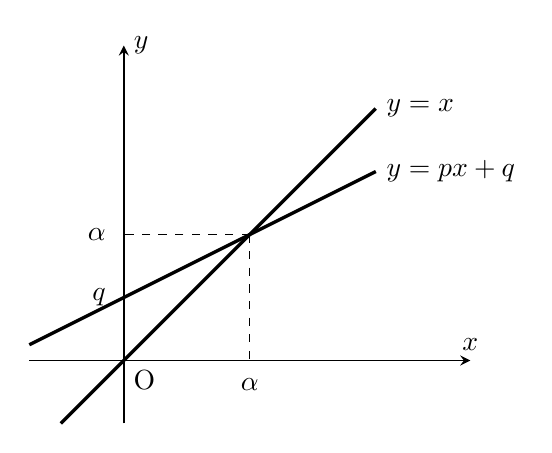
\begin{tikzpicture}[scale=0.8]
    \draw[->,>=stealth,semithick] (-1.5,0)--(5.5,0)node[above]{$x$};
    \draw[->,>=stealth,semithick] (0,-1)--(0,5)node[right]{$y$};
    \draw (0,0)node[below right]{O};

    \draw[very thick,domain=-1:4]
      plot(\x,\x)node[right]{$y=x$};

    \draw[very thick,domain=-1.5:4]
      plot(\x,\x/2+1) node[right] {$y=px+q$};

    % q
    \node[left=3pt] at (0,1) {$q$};

    % 交点から各軸へ点線
    \draw[dashed] (2,2) -- (2,0);
    \draw[dashed] (2,2) -- (0,2);

    % α
    \node[below=3pt] at (2,0) {$\alpha$};
    \node[left=3pt] at (0,2) {$\alpha$};
  \end{tikzpicture}
  \begin{center}
    \BookFigureCaption{直線の交点として捉える\bookterm{fixed}{不動点}}
  \end{center}

  というような状況である.
  この交点$(\alpha,\alpha)$を原点と思ってグラフをみると,この座標平面は$y=px$と$y=x$のグラフが原点から始まって進んでいくようなものに見える.
  言い換えれば等比型\bookterm{recurrence}{漸化式}に帰着させたということである.
  この交点の$x$座標$\alpha$が,更新$f$の\bookterm{fixed}{不動点}である.

  この\bookterm{fixed}{不動点}を知ることによって,複雑な値の変化をより簡素な値の変化に置き換えることができる.
  また,この話から,\,$|p|>1$のときは一般に項数を重ねるにつれて$p$が生み出す等比的な増大が支配的になる一方,\,$|p|<1$のときは$a_n$は$n\to\infty$で$\alpha=\dfrac{q}{1-p}$に収束し,その\bookterm{limit}{極限}値は$q$(と$p$)によって決まることが分かる.例題(2)(\,$p=\frac12$)が$4$に収束するのはこのためである.

  また,\bookterm{characteristic}{特性方程式}型\bookterm{recurrence}{漸化式}には別の解法が存在する.
  以下に示す.
  \begin{align*}
    &a_{n+1}=pa_n+q \tag*{\(\cdots\) (1)}\\
    &a_{n+2}=pa_{n+1}+q \tag*{\(\cdots\) (2)}\\
  \end{align*}
  $(2)-(1)$をし
  \[
    a_{n+2}-a_{n+1}=p(a_{n+1}-a_n)
  \]
  ここで,\,$b_n=a_{n+1}-a_n$と置くと,
  \begin{align*}
    &b_{n+1}=pb_n
  \end{align*}
  このようにすることで,\bookterm{recurrence}{漸化式}は\bookterm{geometric}{等比数列}に帰着する.
  得られた差を初項から足し戻すと、元の\bookterm{sequence}{数列}が求まる。

  こちらの図形的解釈は先程の交点を考えるものとは違う.傾き$p$の平行な2直線$y=px$と$y=px+q$の間には,常に高さ$q$の差が生じている.\,(2)から(1)を引く操作は,この共通の$q$だけを打ち消す操作に対応している.つまり隣接する2つの式を「ずらして引く」ことで,\,$a_n$に無関係な定数項$q$だけを消してしまうのである.これは付録\sectionref{節：差分から始まる離散的な微積分}で扱う\bookterm{difference-operator}{差分}の考え方と同じ発想である.
  これらの前提を元に図示すると

  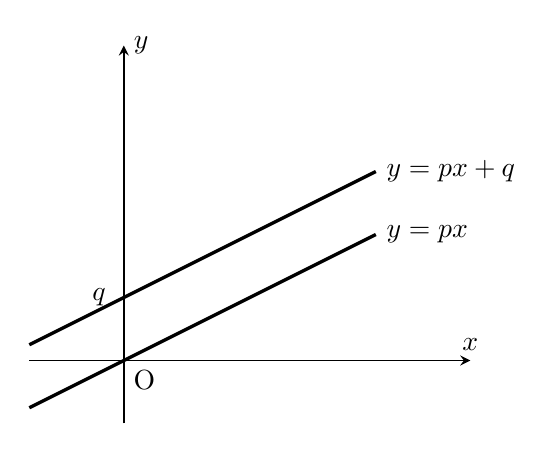
\begin{tikzpicture}[scale=0.8]
    \draw[->,>=stealth,semithick] (-1.5,0)--(5.5,0)node[above]{$x$};
    \draw[->,>=stealth,semithick] (0,-1)--(0,5)node[right]{$y$};
    \draw (0,0)node[below right]{O};

    \draw[very thick,domain=-1.5:4]
      plot(\x,\x/2)node[right]{$y=px$};

    \draw[very thick,domain=-1.5:4]
      plot(\x,\x/2+1) node[right] {$y=px+q$};

    % q
    \node[left=3pt] at (0,1) {$q$};

  \end{tikzpicture}
  \begin{center}
    \BookFigureCaption{定数項の違いを表す平行な直線}
  \end{center}

  常に関数の差が$q$と一定になっていることが図からわかる.

  なお,先ほどの等比的な増大について,初項を\bookterm{fixed}{不動点}に選んだ場合は例外になる.
  \bookterm{fixed}{不動点}から出発すれば値は変わらず,\,$a_n=\alpha$という定\bookterm{sequence}{数列}になるからである.
  式で確かめると,\,$p\ne1$のときは
  \[
    a_n-\alpha=(a_1-\alpha)p^{n-1}
  \]
  である.したがって,\,$|p|>1$でも$a_1=\alpha$ならずれは常に$0$であり,\,$a_1\ne\alpha$の場合に\bookterm{fixed}{不動点}からのずれの絶対値が等比的に増大する.

  今後,\bookterm{characteristic}{特性方程式}を用いた解法を多数扱う.
  \bookterm{characteristic}{特性方程式}は\bookterm{recurrence}{漸化式}を解く中で重要な概念なのである.
  その背景には\bookterm{matrix}{行列}や\bookterm{linear}{線形}代数が深く絡んでいる.

% subsection: 階差等比複合型 \, $\displaystyle a_{n+1}=pa_n+f(n)$

\subsection{\texorpdfstring{階差等比複合型 \, $\displaystyle a_{n+1}=pa_n+f(n)$}{階差等比複合型}}\label{節：階差等比複合型}
  \begin{bookpoint}
    \textbf{同じ更新をする量を引く}\par
    付加項を消すことを目標に,引く式の形と係数を決める.候補を見つける計算と,候補が元の式を満たす確認を区別しよう.
  \end{bookpoint}
  \subsubsection{\texorpdfstring{多項式型 \, $\displaystyle a_{n+1}=pa_n+f(n)$}{多項式型}}
    \bookstep{式の形から、追う量を選ぶ}
    \sectionref*{節：特性方程式型}では,同じ更新をする定数を引いた.
    今回は付加項$f(n)$が$n$によって変わるため,引く量も$n$によって変えてみる.
    \sectionref*{節：補助数列の設計}で述べた方針に従い,同じ更新をする既知の量を探そう.
    本文では$f(n)$が多項式の場合を考える.$p=1$なら\bookterm{difference}{階差}型として和を求められるので,まず$p\ne1$とする.

    \bookstep{引く量を選ぶ}
    $b_n=a_n-g(n)$を等比型にするための条件は
    \[
      g(n+1)=pg(n)+f(n)
    \]
    である.これは,\,$g(n)$自身にも同じ更新をさせるという条件である.
    条件が満たされれば,
    \[
      \begin{array}{rrl}
        &a_{n+1}={}&pa_n+f(n)\\
        -\,)&g(n+1)={}&pg(n)+f(n)\\ \hline
        &a_{n+1}-g(n+1)={}&p\{a_n-g(n)\}
      \end{array}
    \]
    となり,付加項が消える.
    \sectionref*{節：非同次と解の組合せ}で見た「一つの既知の解と\bookterm{homogeneous}{同次}の解に分ける」考え方が,
    ここでは$a_n=g(n)+b_n$として現れている.
    $g(n)$を見つける計算と,残る\bookterm{homogeneous}{同次}の解$b_n$を\bookterm{initial}{初期条件}から選ぶ計算を分けているのである.

    $f(n)$が$m$次式なら,\,$p\ne1$のときは$m$次の多項式
    \[
      g(n)=x_0+x_1n+\cdots+x_mn^m
    \]
    を候補にする.$g(n+1)-pg(n)$の最高次の係数は$(1-p)x_m$である.
    これを$f(n)$の最高次の係数に合わせ,次に一段低い係数を合わせる.
    $1-p\ne0$なので,この順に$x_m,x_{m-1},\ldots,x_0$を決められる.
    未知の係数を比較して求めるこの方法を\bookterm{undetermined}{未定係数法}という.

    例えば$a_{n+1}=2a_n+n-1$では,\,$g(n)=un+v$と置くと
    \[
      u=2u+1,\qquad u+v=2v-1
    \]
    となるので,\,$g(n)=-n$である.
    従って$a_n+n$が2倍される量となる.
    この例の計算は\bookproblemref{practice-basic}{4}{標準問4}で確認する.

    \bookstep{変化を求めて、元の項へ戻す}
    $b_{n+1}=pb_n$を解き,\,$a_n=b_n+g(n)$へ戻す.
    $p\ne0,1$なら
    \[
      a_n=\{a_1-g(1)\}p^{n-1}+g(n)
    \]
    となる.$p=0$なら直接$n\ge2$で$a_n=f(n-1)$と求める.
    一方,\,$p=1$で$f(n)$が$m$次なら,付加項を足し戻す多項式は通常$m+1$次になる.
    例えば$a_{n+1}=a_n+n$では,\,$g(n)=\frac{n(n-1)}2$が同じ更新を満たす.

  \subsubsection{\texorpdfstring{指数型  \, $\displaystyle a_{n+1}=pa_n+q^n$}{指数型}}
    前節では$f(n)$が多項式である場合を扱った.
    ここでは$f(n)$が特に指数関数である場合を扱う.
    指数関数である場合にはもう一つ別の解法が存在する.
    \begin{align*}
      a_{n+1}=pa_n+q^n
    \end{align*}
    以下では$q\ne0$とする($q=0$なら$n\ge1$で$q^n=0$なので等比型になる).
    両辺を$q^n$で割って,
    \begin{align*}
      &\frac{a_{n+1}}{q^n}=\frac{p}{q}\cdot\frac{a_n}{q^{n-1}}+1\\
    \end{align*}
    ここで,\,$b_n=\frac{a_n}{q^{n-1}}$と置くと
    \begin{align*}
      &b_{n+1}=\frac{p}{q}b_n+1
    \end{align*}
    あとは\bookterm{characteristic}{特性方程式}型の\bookterm{recurrence}{漸化式}として解くことになる.
    ただし$p=q$のときは$b_{n+1}=b_n+1$(\bookterm{arithmetic}{等差数列})になり,\bookterm{fixed}{不動点}$\alpha$が存在しない(\sectionref{節：特性方程式型}の例題(3)と同じ状況である).
    この場合は$b_n=b_1+(n-1)$として直接求まる.
    例えば$a_1=1,\,a_{n+1}=2a_n+2^n$(\,$p=q=2$)ならば$b_n=\dfrac{a_n}{2^{n-1}}$が\bookterm{arithmetic}{等差数列}となり,\,$a_n=n\cdot2^{n-1}$が得られる.

% subsection: 対数型 \, $a_{n+1}=pa_n^q$

\subsection{対数型 \, $a_{n+1}=pa_n^q$}
  今までは$a_n$に対する操作は定数倍したり関数が掛けられたりするだけだった.
  しかし,\,$a_n$に指数がついたらどうだろうか.
  この場合はかなり難しい発想の変形が必要である.
  それは対数を取るという操作である.
  実際にやってみよう.
  \[
    a_{n+1}=pa_n^q
  \]
  ただし,対数を取るために$a_n>0$とし,底に選ぶ$p$も$p>0,\,p\ne1$を満たすとする.
  この式について,両辺の対数を取ると
  \begin{align*}
    \log_p{a_{n+1}}&=\log_p{pa_n^q}\\
    &=\log_p{p}+\log_p{a_n^q}\\
    &=q\log_p{a_n}+1
  \end{align*}
  $b_n=\log_p{a_n}$とおくと,
  \begin{align*}
    b_{n+1}=qb_n+1
  \end{align*}
  あとはただの特性方程式型の問題である.
  底をいくらにするかは自由だが$p$に関連する数だと扱いやすい.
  たとえば$p=k^m$の時は$k$でとっておくことが多い.
  作問者側は解答がシンプルな形になるようにするため,より小さい底を取ることで答えが求めやすくなる.

  また,対数の強みは積を和に,商を差にできるところにある.
  漸化式が全て積や商のみで表される場合にその強みが現れる.
  これはここで解説するよりも演習問題を通して経験するほうがわかりやすいと判断したため,この内容は(2)で取り扱っている.

  \noindent\textbf{【例題】}
  \begin{enumerate}[label=(\arabic*),parsep=3pt]
    \item $\displaystyle a_1=2,\quad a_{n+1}=2a_n^2$
    \item $\displaystyle a_1=\frac{1}{2},\quad a_{n+1}=\frac{1}{a_n}$
    \item $\displaystyle a_1=1,\quad a_{n+1}=2^na_n$
    \item $\displaystyle a_1=5,\quad a_{n+1}=a_n^2-2a_n+2$
    \item $\displaystyle a_1=2,\quad a_{n+1}=\frac{a_n^2}{2^n}$
    \item $\displaystyle a_1=1,\quad a_{n+1}=(n+1)a_n$
  \end{enumerate}

  \noindent\textbf{【方針】}
  \begin{enumerate}[label=(\arabic*),parsep=3pt]
    \item 両辺の底を$2$とする対数を取り,\,$b_n=\log_2a_n$とおいて一次の漸化式に変形します.その結果,漸化式は特性方程式型になります.
    \item 一見すると分数型(後述)のように見えますが,対数型として解くことができます.
    \item $f(n)=2^n$が指数関数なので,対数を取ると和の形に帰着できます.
    \item うまく変形すると対数型になります.
    \item 両辺の対数を取ると,二次の漸化式が一次の漸化式に変わり,さらに等差数列の和を使って解くことができます.
    \item 階比型に見えますが,対数型としても解けます.
  \end{enumerate}

  \noindent\textbf{【解答】}
  \begin{enumerate}[label=(\arabic*),parsep=3pt]
    \item $\displaystyle a_n=2^{2^{n}-1}$
    \item $a_n=2^{(-1)^{n}}$
    \item $a_n=2^{\frac{n(n-1)}{2}}$
    \item $a_n=2^{2^n}+1$
    \item $\displaystyle a_n=2^{n-1}-n+1$
    \item $a_n=n!$
  \end{enumerate}

  \noindent\textbf{【解法】}
  \begin{enumerate}[label=(\arabic*),parsep=3pt]
    \item $\displaystyle a_1=2,\quad a_{n+1}=2a_n^2$\\
          両辺の底を$2$とする対数を取ると,
          \begin{align*}
            \log_2a_{n+1}
              &=\log_2{2a_n^2}\\
              &=\log_2{2}+\log_2{a_n^2}\\
              &=2\log_2{a_n}+1
          \end{align*}
          ここで
          \[
            b_n=\log_2a_n
          \]
          とおくと,
          \begin{align*}
            &b_{n+1}=2b_n+1\\
            &b_{n+1}+1=2(b_n+1)
          \end{align*}
          ここで
          \[
            c_n=b_n+1
          \]
          とおくと,
          \[
            c_{n+1}=2c_n
          \]
          $c_1$は,
          \[
            c_1=b_1+1=\log_2{a_1}+1=\log_2{2}+1=1+1=2
          \]
          従って,
          \begin{align*}
            &c_n=2\cdot2^{n-1}=2^n\\
            &b_n+1=2^n\\
            &b_n=2^n-1\\
            &a_n=2^{2^{n}-1}
          \end{align*}
    \item $\displaystyle a_1=\frac12,\quad a_{n+1}=\frac{1}{a_n}$\\
          与式の両辺の底を2とする対数を取ると,
          \begin{align*}
            &\log_2{a_{n+1}}=\log_2{\frac{1}{a_n}}\\
            &\log_2{a_{n+1}}=\log_2{1}-\log_2{a_n}\\
            &\log_2{a_{n+1}}=-\log_2{a_n}\\
            &\log_2{a_n}=\log_2{a_1}(-1)^{n-1}\\
            &\log_2{a_n}=\log_2{\frac{1}{2}}(-1)^{n-1}\\
            &\log_2{a_n}=(-1)^{n}\\
            &\therefore \quad a_n=2^{(-1)^{n}}
          \end{align*}
    \item $\displaystyle a_1=1,\quad a_{n+1}=2^na_n$\\
          両辺の自然対数を取ると
          \[
            \log a_{n+1}=n\log2+\log a_n
          \]
          したがって
          \begin{align*}
            \log a_n&=\log a_1+\sum_{k=1}^{n-1} k\log2\\
            &=\frac{(n-1)n}{2}\log2\\
            &\therefore \quad a_n=2^{\frac{n(n-1)}{2}}
          \end{align*}
    \item $\displaystyle a_1=5,\quad a_{n+1}=a_n^2-2a_n+2$\\
          与式を変形して
          \[
            a_{n+1}-1=(a_n-1)^2
          \]
          両辺の底を2とする対数を取ると,
          \begin{align*}
            &\log_2{(a_{n+1}-1)}=\log_2{(a_n-1)^2}\\
            &\log_2{(a_{n+1}-1)}=2\log_2{(a_n-1)}\\
            &\log_2{(a_n-1)}=2^{n-1}\cdot\log_2{(a_1-1)}\\
            &\log_2{(a_n-1)}=2^{n-1}\cdot\log_2{4}\\
            &\log_2{(a_n-1)}=2^{n}\\
            &a_n-1=2^{2^{n}}\\
            &\therefore \quad a_n=2^{2^{n}}+1
          \end{align*}
    \item $\displaystyle a_1=2,\quad a_{n+1}=\frac{a_n^2}{2^n}$\\
          両辺を底を2とする自然体数を取って
          \[
            equation
          \]
    \item $\displaystyle a_1=1,\quad a_{n+1}=(n+1)a_n$\\
          両辺の自然対数を取って,
          \[
            \log a_{n+1}=\log{n+1}+\log a_n
          \]
          したがって
          \begin{align*}
            \log a_n&=\log a_1 + \log{2}+\cdots+ \log{n}\\
            &=\log 1 + \log{2}+\cdots +\log{n}\\
            &=\log n!\\
            &\therefore \quad a_n=n!
          \end{align*}
  \end{enumerate}
  \noindent\textbf{【補足】}

  (3)では底を自然対数としたが,底は任意の値で構わない.


% parent file: 分数型
\subsection{分数型}\label{節：分数型}
\begin{bookpoint}
  \textbf{分母を簡単にする量を選ぶ}\par
  逆数,または\bookterm{fixed}{不動点}からの二つの差の比を追う.
  分母が零になる初期値と定数解の分岐を確かめてから,置き換えを使う.
\end{bookpoint}
% subsubsection: 逆数型  \, $\displaystyle a_{n+1}=\frac{pa_n}{qa_n+r}$

\subsubsection{\texorpdfstring{逆数型  \, $\displaystyle a_{n+1}=\frac{pa_n}{qa_n+r}$}{逆数型}}
    では逆数型の漸化式について扱っていこう.
    分子が$a_n$の定数倍であることに注目する.
    逆数を取れば,分母にあった一次式を$a_n$で割り,定数と$\frac1{a_n}$の和に分けられる.
    以下では,$p\ne0$かつ$a_n\ne0$であり,$qa_n+r\ne0$として議論する.
    実際に見せよう.
    \begin{align*}
      &a_{n+1}=\frac{pa_n}{qa_n+r}
    \end{align*}
      両辺の逆数を取って
    \begin{align*}
      &\frac{1}{a_{n+1}}=\frac{qa_n+r}{pa_n}\\
      &\frac{1}{a_{n+1}}=\frac{q}{p}+\frac{r}{p}\cdot\frac{1}{a_n}
    \end{align*}
    $\displaystyle \frac{1}{a_n}=b_n$と置くと
    \begin{align*}
      &b_{n+1}=\frac{r}{p}b_n+\frac{q}{p}
    \end{align*}
    このようにすることで,特性方程式型の漸化式に帰着できる.

    \noindent \bookblocklink{example-reciprocal-1}{problem}{answer}{【例題】}
    \begin{enumerate}[label=(\arabic*),parsep=3pt,format=\bookitemlink{example-reciprocal-1}{problem}{answer}]
      \item $\displaystyle a_1=1,\, a_{n+1}=\frac{a_n}{a_n+1}$
      \item $\displaystyle a_1=1,\, a_{n+1}=\frac{-a_n}{2a_n+1}$
    \end{enumerate}

    \noindent\bookblocklink{example-reciprocal-1}{hint}{problem}{【方針】}
    \begin{enumerate}[label=(\arabic*),parsep=3pt,format=\bookitemlink{example-reciprocal-1}{hint}{problem}]
      \item とにかく基本に忠実に解きましょう.
      \item 逆数を取って一次の漸化式に帰着させましょう.
    \end{enumerate}

    \noindent\bookblocklink{example-reciprocal-1}{answer}{problem}{【解答】}
    \begin{enumerate}[label=(\arabic*),parsep=3pt,format=\bookitemlink{example-reciprocal-1}{answer}{problem}]
      \item $\displaystyle a_n=\frac{1}{n}$
      \item $\displaystyle a_n=\frac{1}{2(-1)^{n-1}-1}$
    \end{enumerate}

    \noindent\bookblocklink{example-reciprocal-1}{solution}{problem}{【解法】}
    \begin{enumerate}[label=(\arabic*),parsep=3pt,format=\bookitemlink{example-reciprocal-1}{solution}{problem}]
      \item $\displaystyle a_1=1,\, a_{n+1}=\frac{a_n}{a_n+1}$\\
            両辺の逆数を取って,
            \begin{align*}
              &\frac{1}{a_{n+1}}=\frac{a_n+1}{a_n}=1+\frac{1}{a_n}
            \end{align*}
            $b_n=\dfrac{1}{a_n}$と置くと
            \begin{align*}
              &b_{n+1}=b_n+1,\quad b_1=\frac{1}{a_1}=1\\
              &\therefore \quad b_n=1+(n-1)\cdot1=n\\
              &\therefore \quad a_n=\frac{1}{b_n}=\frac{1}{n}
            \end{align*}
      \item $\displaystyle a_1=1,\, a_{n+1}=\frac{-a_n}{2a_n+1}$\\
            両辺の逆数を取って,
            \begin{align*}
              &\frac{1}{a_{n+1}}=\frac{2a_n+1}{-a_n}=-2-\frac{1}{a_n}
            \end{align*}
            $b_n=\dfrac{1}{a_n}$と置くと,
            \begin{align*}
              &b_{n+1}=-b_n-2,\quad b_1=1
            \end{align*}
            特性方程式型として$\alpha$を求めると,
            \[
              \alpha=-\alpha-2 \ \Leftrightarrow\ \alpha=-1
            \]
            なので,\,$c_n=b_n+1$と置くと,
            \begin{align*}
              &c_{n+1}=-c_n,\quad c_1=b_1+1=2\\
              &\therefore \quad c_n=2\cdot(-1)^{n-1}\\
              &\therefore \quad b_n=c_n-1=2(-1)^{n-1}-1\\
              &\therefore \quad a_n=\frac{1}{b_n}=\frac{1}{2(-1)^{n-1}-1}
            \end{align*}
    \end{enumerate}

% subsubsection: 1次分数型  \, $\displaystyle a_{n+1}=\frac{pa_n+q}{ra_n+s}$

\subsubsection{\texorpdfstring{1次分数型  \, $\displaystyle a_{n+1}=\frac{pa_n+q}{ra_n+s}$}{1次分数型}}\label{節：1次分数型}
    先程の逆数型の一般化と言える漸化式である,\,1次分数型の漸化式について考えていこう.
    以下では,\, $r\ne0$,\, $ps-qr\ne0$とし,もとの漸化式の分母が$0$にならないものとして議論を進める.

    数学における基本的な指針として,既知の形に帰着させるというものがある.
    本書で言う,"きれい"な形にするということである.
    今回の漸化式で,分子の定数項$q$がなければ,つまりは,
    \[
      a_{n+1}=\frac{pa_n+q}{ra_n+s} \Leftrightarrow b_{n+1}=\frac{tb_n}{u b_n+v}
    \]
    となるような$b_n$と$t,u,v$の組があれば逆数型として解くことができる.
    そこで,分子の定数項を消し,逆数型に帰着させることを目標にしよう.

    \,\sectionref{節：特性方程式型}では,数列の各項から同じ定数を引くことで定数項を消した.
    今回もそのアイデアを使い,\, $b_n=a_n-\alpha$と置いてみよう.
    ただし,ここでは$\alpha$をまだ決めず,変形後の分子の定数項が消えるように選ぶ.
    $a_n=b_n+\alpha$を代入すると,
    \begin{align*}
      b_{n+1}-\alpha &=\frac{p(b_n+\alpha)+q}{r(b_n+\alpha)+s}\\
      b_{n+1} &=\frac{p(b_n+\alpha)+q}{r(b_n+\alpha)+s}-\alpha\\
      &=\frac{p(b_n+\alpha)+q-\alpha\{r(b_n+\alpha)+s\}}
        {r(b_n+\alpha)+s}\\
      &=\frac{(p-r\alpha)b_n+p\alpha+q-r\alpha^2-s\alpha}
        {rb_n+r\alpha+s}
    \end{align*}
    となる.したがって,
    \[
      p\alpha+q-r\alpha^2-s\alpha=0
    \]
    となるように$\alpha$を選べば,
    \[
      b_{n+1}=\frac{(p-r\alpha)b_n}{rb_n+r\alpha+s}
    \]
    という逆数型に帰着できる.
    定数項を消すための条件は,
    \[
      r\alpha^2+(s-p)\alpha-q=0
      \quad\Longleftrightarrow\quad
      \alpha=\frac{p\alpha+q}{r\alpha+s}
    \]
    と書けるので,この$\alpha$はもとの漸化式の不動点でもある.
    なお,\, $r\alpha+s=0$なら上の方程式から$p\alpha+q=0$も成り立ち,\, $ps-qr=0$となって仮定に反するので,この分母は$0$ではない.

    ここまでで逆数型として解くことができるが,定数項を消せる値を求める問題は,
    \[
      rx^2+(s-p)x-q=0
    \]
    という二次方程式を解く問題に帰着した.
    この方程式が異なる2つの実数解$\alpha,\beta$を持つなら,その左辺は
    \[
      rx^2+(s-p)x-q=r(x-\alpha)(x-\beta)
    \]
    と因数分解できる.
    $\alpha,\beta$は別々に選ぶ定数ではなく,もとの漸化式の係数から決まる,同じ二次方程式の二つの解なのである.
    そして,どちらの解も定数項を消す条件を満たすので,\, $a_n-\alpha$と$a_n-\beta$のどちらについても,同じ変形ができる.
    先ほどの逆数型の式を,もとの$a_n$を使って書き直すと,
    \begin{align*}
      a_{n+1}-\alpha
      &=\frac{p-r\alpha}{ra_n+s}(a_n-\alpha),\\
      a_{n+1}-\beta
      &=\frac{p-r\beta}{ra_n+s}(a_n-\beta)
    \end{align*}
    となる.

    この二つの式から,さらに単純な法則を取り出せないだろうか.
    それぞれの差に掛かる倍率には$a_n$が含まれているので,差そのものは一般には等比数列にならない.
    しかし,二つの倍率には同じ分母$ra_n+s$が現れている.
    そこで二つの式の比を取れば,この分母が消え,一定の倍率だけが残りそうである.

    初項が$\alpha$または$\beta$なら定数数列になるので,先に扱っておこう.
    以下では初項がどちらの不動点とも異なる場合を考える.
    また,\, $p-r\beta=0$なら不動点の条件から$q=s\beta$となり,\, $ps-qr=0$となって仮定に反する.
    よって,\, $p-r\beta\ne0$であり,上の式から$a_n\ne\beta$なら$a_{n+1}\ne\beta$である.
    初項から順に考えると,すべての項で$a_n\ne\beta$なので,二つの差の比を取ることができる.
    実際に,
    \begin{align*}
      \frac{a_{n+1}-\alpha}{a_{n+1}-\beta}
      &=\cfrac{\displaystyle
        \frac{(p-r\alpha)(a_n-\alpha)}{ra_n+s}}
        {\displaystyle
        \frac{(p-r\beta)(a_n-\beta)}{ra_n+s}}\\
      &=\frac{p-r\alpha}{p-r\beta}
        \frac{a_n-\alpha}{a_n-\beta}
    \end{align*}
    となる.
    したがって,二つの差の比は,項が一つ進むごとに一定の倍率$\dfrac{p-r\alpha}{p-r\beta}$で変化する.
    分子の定数項を消せる二つの式を比べることで,等比数列の法則を見つけられたのである.

    ここで
    \[
      b_n=\frac{a_n-\alpha}{a_n-\beta}
    \]
    と置けば,
    \[
      b_{n+1}
      =
      \frac{p-r\alpha}{p-r\beta}b_n
    \]
    となる.したがって,\,$b_n$は等比数列である.
    $\alpha$と$\beta$の大小関係は,解の大小関係を要求されていないことから自由に選んでよい.
    つまり,\,1次分数型漸化式では,
    \[
      a_{n+1}=\frac{pa_n+q}{ra_n+s}
    \]
    という複雑な形をそのまま扱うのではなく,
    \[
      \frac{a_n-\alpha}{a_n-\beta}
    \]
    という「$\alpha,\beta$からの距離の比」に置き換えることで,
    等比数列に変えることができる.

    そして,\,$\alpha,\beta$は,
    \[
      rx^2+(s-p)x-q=0
    \]
    の異なる2解として自然に現れる.
    
    したがって\,$\alpha,\beta$は,もとの漸化式の$a_n$を形式的に$\alpha,\beta$に置き換えたときにも値が変化しない数,すなわち不動点である.
    
    議論が長くなったので,ここで解法をまとめておこう.
    \[
      a_{n+1}=\frac{pa_n+q}{ra_n+s} 
    \]
    の形で表される漸化式に対して,ただし$ps-qr\ne0$とし,
    $r\ne0$とする.また,以下では$a_n\ne-\dfrac sr$(漸化式の分母が$0$にならないこと)を仮定する.
    さらに,$a_1\ne\beta$とする.
    \[
      x= \frac{px+q}{rx+s} \Leftrightarrow rx^2+(s-p)x-q=0
    \]
    を解き,その異なる2解を$\alpha,\beta$とする.
    ここで,
    \[
      b_n=\frac{a_n-\alpha}{a_n-\beta}
    \]
    と置く.
    すると,
    \begin{align*}
      b_{n+1}&=\frac{a_{n+1}-\alpha}{a_{n+1}-\beta}\\
      &=\cfrac{\displaystyle\frac{pa_n+q}{ra_n+s}-\alpha}{\displaystyle\frac{pa_n+q}{ra_n+s}-\beta}\\
      &=\frac{pa_n+q-\alpha(ra_n+s)}{pa_n+q-\beta(ra_n+s)}\\
      &=\frac{(p-r\alpha)a_n+q-s\alpha}{(p-r\beta)a_n+q-s\beta}
    \end{align*}
    ここで,\,$\alpha$は
    \[
      r\alpha^2+(s-p)\alpha-q=0
    \]
    を満たすから,
    \[
      q-s\alpha=-\alpha(p-r\alpha)
    \]
    である.
    したがって,
    \[
      (p-r\alpha)a_n+q-s\alpha
      =(p-r\alpha)(a_n-\alpha)
    \]
    同様に,\,$\beta$について
    \[
      (p-r\beta)a_n+q-s\beta
      =(p-r\beta)(a_n-\beta)
    \]
    である.
    よって,
    \begin{align*}
      b_{n+1}&=\frac{(p-r\alpha)(a_n-\alpha)}{(p-r\beta)(a_n-\beta)}\\
      &=\frac{p-r\alpha}{p-r\beta}\frac{a_n-\alpha}{a_n-\beta}\\
      &=\frac{p-r\alpha}{p-r\beta}b_n
    \end{align*}
    したがって,
    \[
      b_{n+1}=\frac{p-r\alpha}{p-r\beta}b_n
    \]
    となり,\,$b_n$は等比数列である.
    初項
    \[
      b_1=\frac{a_1-\alpha}{a_1-\beta}
    \]
    を用いれば,
    \[
      b_n=\frac{a_1-\alpha}{a_1-\beta}\left(\frac{p-r\alpha}{p-r\beta}\right)^{n-1} \tag*{\(\cdots\) (＊)}
    \]
    となる.
    最後に,
    \[
      b_n=\frac{a_n-\alpha}{a_n-\beta}
    \]
    から$a_n$を求める.
    \begin{align*}
      b_n(a_n-\beta)&=a_n-\alpha\\
      (b_n-1)a_n&=\beta b_n-\alpha\\
      a_n=\frac{\beta b_n-\alpha}{b_n-1}
    \end{align*}
    (＊)を代入して$a_n$を求めることができる.

    なお,$rx^2+(s-p)x-q=0$が重解$\alpha$を持つ場合は,$\beta$と異なる2つの不動点を取れないため,上の議論はそのまま使えない.
    このときは$\alpha=\dfrac{p-s}{2r}$,すなわち$s=p-2r\alpha$が成り立つため,
    \[
      c=p-r\alpha=r\alpha+s\ne0
    \]
    とおくと,
    \[
      a_{n+1}-\alpha
      =\frac{c(a_n-\alpha)}{r(a_n-\alpha)+c}
    \]
    となる.したがって,
    \[
      \frac{1}{a_{n+1}-\alpha}
      =\frac{1}{a_n-\alpha}+\frac{r}{c}
    \]
    であるから,右辺も含めて$\displaystyle \frac{1}{a_n-\alpha}$について考えれば等差数列に帰着できる.
    ここで$b_n=a_n-\alpha$とおくと,
    \[
      b_{n+1}=\frac{cb_n}{rb_n+c}
    \]
    という逆数型漸化式に帰着する(先ほどの一般式で$\beta=\alpha$とした場合に対応する).したがって両辺の逆数を取れば
    \[
      \frac1{b_{n+1}}=\frac1{b_n}+\frac rc
    \]
    という等差数列が得られ,ここから$a_n$を求めることができる(具体的な計算は例題(3)を参照).

    \noindent \bookblocklink{example-mobius-1}{problem}{answer}{【例題】}
    \begin{enumerate}[label=(\arabic*),parsep=3pt,format=\bookitemlink{example-mobius-1}{problem}{answer}]
      \item $\displaystyle a_1=3,\, a_{n+1}=\frac{2a_n+1}{a_n+2}$
      \item $\displaystyle a_1=0,\, a_{n+1}=\frac{a_n+4}{a_n+1}$
      \item $\displaystyle a_1=5,\, a_{n+1}=\dfrac{4a_{n}-9}{a_{n}-2}$
      \item $\displaystyle a_1=1,\, a_{n+1}=1+\frac{1}{a_n}$
    \end{enumerate}

    \noindent\bookblocklink{example-mobius-1}{hint}{problem}{【方針】}
    \begin{enumerate}[label=(\arabic*),parsep=3pt,format=\bookitemlink{example-mobius-1}{hint}{problem}]
      \item 最も基本的な例です.先程の議論に倣って解きましょう.
      \item 同様に不動点$\alpha,\beta$を求めましょう.今回は片方が負の値になります.
      \item 今回は不動点の方程式が重解になります.\,$\dfrac{a_n-\alpha}{a_n-\beta}$は使えないので,\,$b_n=a_n-\alpha$と置いてから逆数型に帰着させる別の手法を使います.
      \item このような形も一次分数型です.解と係数の関係を活用して解きましょう.
    \end{enumerate}

    \noindent\bookblocklink{example-mobius-1}{answer}{problem}{【解答】}
    \begin{enumerate}[label=(\arabic*),parsep=3pt,format=\bookitemlink{example-mobius-1}{answer}{problem}]
      \item $\displaystyle a_n=\frac{2\cdot3^{n-1}+1}{2\cdot3^{n-1}-1}$
      \item $\displaystyle a_n=\frac{2\left(3^{n-1}+(-1)^n\right)}{3^{n-1}-(-1)^n}$
      \item $a_{n}=\dfrac{6n-1}{2n-1}$
      \item $\displaystyle a_n=\cfrac{\left(\cfrac{1-\sqrt{5}}{2}\right)^{n+1}-\left(\cfrac{1+\sqrt{5}}{2}\right)^{n+1}}{\left(\cfrac{1-\sqrt{5}}{2}\right)^n-\left(\cfrac{1+\sqrt{5}}{2}\right)^n}$
    \end{enumerate}

    \noindent\bookblocklink{example-mobius-1}{solution}{problem}{【解法】}
    \begin{enumerate}[label=(\arabic*),parsep=3pt,format=\bookitemlink{example-mobius-1}{solution}{problem}]
      \item $\displaystyle a_1=3,\, a_{n+1}=\frac{2a_n+1}{a_n+2}$\\
            不動点の方程式は
            \[
              x=\frac{2x+1}{x+2}
            \]
            であるから,その解をそれぞれ$\alpha,\beta$とすると\,$\alpha=1,\ \beta=-1$と取れる.
            このとき,
            \[
              b_n=\frac{a_n-1}{a_n+1}
            \]
            と置くと,
            \begin{align*}
              b_{n+1}&=\frac{a_{n+1}-1}{a_{n+1}+1}\\
              &=\cfrac{\cfrac{2a_n+1}{a_n+2}-1}{\cfrac{2a_n+1}{a_n+2}+1}\\
              &=\frac{2a_n+1-(a_n+2)}{2a_n+1+(a_n+2)}\\
              &=\frac{a_n-1}{3a_n+3}\\
              &=\frac{1}{3}\cdot \frac{a_n-1}{a_n+1}
            \end{align*}
            $\displaystyle b_1=\frac{a_1-1}{a_1+1}=\frac{2}{4}=\frac{1}{2}$から,
            \begin{align*}
              b_{n}=\frac{1}{2}\cdot\left(\frac{1}{3}\right)^{n-1}\\
              \therefore \quad b_n=\frac{1}{2\cdot3^{n-1}}
            \end{align*}
            最後に
            \[
              b_n=\frac{a_n-1}{a_n+1}
            \]
            を$a_n$について解くと,
            \begin{align*}
              &b_n(a_n+1)=a_n-1\\
              &(b_n-1)a_n=-1-b_n\\
              &a_n=\frac{1+b_n}{1-b_n}
            \end{align*}
            \[
              b_n=\frac{1}{2\cdot3^{n-1}}
            \]
            を代入して整理すれば,
            \[
              a_n=\frac{2\cdot3^{n-1}+1}{2\cdot3^{n-1}-1}
            \]
            を得る.
      \item $\displaystyle a_1=0,\, a_{n+1}=\frac{a_n+4}{a_n+1}$\\
            不動点の方程式は
            \[
              x=\frac{x+4}{x+1}
            \]
            であるから,その解をそれぞれ$\alpha,\beta$とすると\,$\alpha=2,\ \beta=-2$と取れる.
            このとき,
            \[
              \frac{p-r\alpha}{p-r\beta}=\frac{1-2}{1+2}=-\frac13
            \]
            なので,
            \[
              b_n=\frac{a_n-2}{a_n+2}
            \]
            と置くと,
            \begin{align*}
              &b_{n+1}=-\frac13 b_n,\quad b_1=\frac{a_1-2}{a_1+2}=\frac{-2}{2}=-1\\
              &\therefore \quad b_n=(-1)\left(-\frac13\right)^{n-1}=\frac{(-1)^n}{3^{n-1}}
            \end{align*}
            \[
              b_n=\frac{a_n-2}{a_n+2}
            \]
            を$a_n$について解くと,
            \[
              a_n=\frac{2(1+b_n)}{1-b_n}
            \]
            となるので,
            \[
              b_n=\frac{(-1)^n}{3^{n-1}}
            \]
            を代入し,分母分子に$3^{n-1}$を掛けて整理すると,
            \[
              a_n=\frac{2\left(3^{n-1}+(-1)^n\right)}{3^{n-1}-(-1)^n}
            \]
            を得る.
      \item $\displaystyle a_1=5,\, a_{n+1}=\dfrac{4a_{n}-9}{a_{n}-2}$
            不動点の方程式は
            \[
              x=\frac{4x-9}{x-2}
            \]
            であるから,その解は3.
            \[
            b_n=a_n-3
            \]
            とおくと,
            \begin{align*}
              b_{n+1}&=a_{n+1}-3\\
              &=\dfrac{4a_{n}-9}{a_{n}-2}-3\\
              &=\dfrac{a_{n}-3}{a_{n}-2}\\
              &=\dfrac{b_{n}}{b_{n}+1}
            \end{align*}
            逆数を取って
            \begin{align*}
              \frac{1}{b_{n+1}}&=\dfrac{b_{n}+1}{b_{n}}
            \end{align*}
            $b_1=a_1-3=2$,すなわち$\dfrac1{b_1}=\dfrac12$より,
            \begin{align*}
              &\frac{1}{b_n}=\frac{1}{2}+(n-1)\cdot 1\\
              &\frac{1}{b_n}=\frac{2n-1}{2}\\
              &b_n=\frac{2}{2n-1}\\
              &a_n-3=\frac{2}{2n-1}\\
              &a_n=\frac{6n-1}{2n-1}
            \end{align*}
      \item $\displaystyle a_1=1,\, a_{n+1}=1+\frac{1}{a_n}$\\
            式を変形して
            $\displaystyle a_1=1,\, a_{n+1}=\frac{a_n+1}{a_n}$
            不動点の方程式は
            \[
              x=\frac{x+1}{x}\tag*{\(\cdots\) (1)}
            \]
            であるから,その解をそれぞれ$\alpha,\beta$とすると
            \[
              \alpha=\frac{1+\sqrt{5}}{2},\ \beta=\frac{1-\sqrt{5}}{2}
            \]
            ここで(1)について,その解$\alpha,\beta$では
            \[
              \alpha+\beta=1,\, \quad \alpha\beta=-1\tag*{\(\cdots\) (2)}
            \]
            が解と係数の関係から成り立つ.したがって,
            \begin{align*}
              b_{n+1}&=\frac{a_{n+1}-\alpha}{a_{n+1}-\beta}\\
              &=\cfrac{\cfrac{a_n+1}{a_n}-\alpha}{\cfrac{a_n+1}{a_n}-\beta}\\
              &=\frac{a_n+1-\alpha a_n}{a_n+1-\beta a_n}\\
              &=\frac{(1-\alpha)a_n+1}{(1-\beta)a_n+1}\tag*{\(\cdots\) (3)}
            \end{align*}
            (2)より,(3)は
            \begin{align*}
              \frac{(1-\alpha)a_n+1}{(1-\beta)a_n+1}&=\frac{\beta a_n+1}{\alpha a_n+1}\\
              &=\frac{\beta a_n-\alpha\beta}{\alpha a_n-\alpha\beta}\\
              &=\frac{\beta (a_n-\alpha)}{\alpha (a_n-\beta)}\\
              &=\frac{\beta}{\alpha}b_n
            \end{align*}
            よって,
            \[
              b_{n+1}=\frac{\beta}{\alpha}b_n
            \]
            初項$b_1$は,
            \begin{align*}
              b_1=\frac{a_1-\alpha}{a_1-\beta}=\frac{1-\alpha}{1-\beta}=\frac{\beta}{\alpha}
            \end{align*}
            したがって,
            \[
              b_n=\left(\frac{\beta}{\alpha}\right)^n
            \]
            次に
            \[
              b_{n}=\frac{a_{n}-\alpha}{a_{n}-\beta}
            \]
            を$a_n$について解くと,
            \[
              a_{n}=\frac{\beta b_{n}-\alpha}{b_{n}-1}
            \]
            したがって,
            \begin{align*}
              a_{n}&=\cfrac{\beta \left(\cfrac{\beta}{\alpha}\right)^n-\alpha}{\left(\cfrac{\beta}{\alpha}\right)^n-1}  \\
              &=\frac{\beta^{n+1}-\alpha^{n+1}}{\beta^n-\alpha^n}\\
              &=\cfrac{\left(\cfrac{1-\sqrt{5}}{2}\right)^{n+1}-\left(\cfrac{1+\sqrt{5}}{2}\right)^{n+1}}{\left(\cfrac{1-\sqrt{5}}{2}\right)^n-\left(\cfrac{1+\sqrt{5}}{2}\right)^n}
            \end{align*}        
    \end{enumerate}
  余談にはなるが,最後の問題はフィボナッチ数列の2項間の比の極限値は黄金比$\dfrac{1+\sqrt{5}}{2}$に一致する.
  実際,\,$a_n=\dfrac{F_{n+1}}{F_n}$(ただし$F_n$は$F_1=F_2=1$から定まるフィボナッチ数列)であることが,同じ漸化式$a_{n+1}=1+\dfrac1{a_n}$から確かめられる.
  また,ここから派生したリュカ数列も同じ特性方程式$x^2=x+1$を持ち,隣接項の比が同じ黄金比に収束する.
  一方,同様に漸化式から派生する数列にトリボナッチ数列があるが,こちらは特性方程式が3次$(x^3=x^2+x+1)$になり,隣接項の比の極限値(トリボナッチ定数,約$1.839$)は黄金比とは異なる.
  これらは本書の趣旨から外れてしまうため割愛する.

  加えて,このタイプの漸化式は帰納法によって示すことが比較的容易なパターンが存在する.
  例えば(3)は解答の一般項から分かるように,分母分子それぞれが一次関数の形で書かれているため,想像しやすい.
  $a_1$から$a_3$ぐらいまでを求めさせてから帰納法で示させるような誘導問題が出た時は帰納法を使って解くことも視野に入れておくといいだろう.
  以下にその例を示す.\\
    \noindent\bookblocklink{example-mobius-2}{problem}{answer}{【例題】}
    \begin{quote}
      以下の漸化式
      \[
        a_1=5,\, a_{n+1}=\dfrac{4a_{n}-9}{a_{n}-2}
      \]
      を満たす数列$a_n$の一般項を帰納法を用いて求めよ.
    \end{quote}
    \bookblocklink{example-mobius-2}{hint}{problem}{【方針】}
    \begin{quote}
      実験的に代入計算をしてみると,
      \[
        a_1=\frac{5}{1},\,a_2=\frac{11}{3},\,a_3=\frac{17}{5},\,a_4=\frac{23}{7},\,a_5=\frac{29}{9}
      \]
      となる.分母が2ずつ,分子が6づつ増えていることから,一般項は
      \[
        a_n=\frac{6n-1}{2n-1}
      \]
      と予想する.
    \end{quote}
    \bookblocklink{example-mobius-2}{answer}{problem}{【解答】}
    \begin{quote}
      一般項$a_n$が
      \[
        a_n=\frac{6n-1}{2n-1}
      \]
      であることを示す.\\
      $n=1$の時,
      \[
        \frac{6-1}{2-1}=5
      \]
      よって成立する.\\
      ある正の整数$k$について,$n=k$が成り立つと仮定する.このとき,
      \[
        n=k+1
      \]
      のとき,
      \begin{align*}
        a_{k+1}&=\frac{4a_{k}-9}{a_{k}-2}\\
        &=\cfrac{4\cdot \cfrac{6k-1}{2k-1}-9}{\cfrac{6k-1}{2k-1}-2}\\
        &=\frac{4(6k-1)-9(2k-1)}{6k-1-2(2k-1)}\\
        &=\frac{6k+5}{2k+1}\\
        &=\frac{6(k+1)-1}{2(k+1)-1}
      \end{align*}
      したがって,$n=k+1$でも成立する.
      以上より
      \[
        a_n=\frac{6n-1}{2n-1}
      \]
      が示された.\qed

  \end{quote}


% subsubsection: 極形式による図形的解釈

\subsubsection{極形式による図形的解釈}
  \BookFigMobius

  図では,点$a_n$と二つの\bookterm{fixed}{不動点}$\alpha,\beta$を結ぶ線分を描いた.
  上の線分の長さを下の線分の長さで割ると,
  \[
    \frac{|a_n-\alpha|}{|a_n-\beta|}
    =\left|\frac{a_n-\alpha}{a_n-\beta}\right|
    =|b_n|
  \]
  となる.また,二つの線分の向きの差は,
  $b_n$の\bookterm{argument}{偏角}$\arg b_n$に対応する.
  したがって,図で見ている\textbf{長さの比と角度の差}は,
  計算で導入する一つの複素数$b_n$の絶対値と\bookterm{argument}{偏角}に他ならない.
  さらに$b_{n+1}=\lambda b_n$となったときは,
  長さの比が$|\lambda|$倍され,角度の差が$\arg\lambda$だけ増える.
  特に$|\lambda|=1$なら,長さの比を保ったまま\bookterm{argument}{偏角}だけが変わり,
  \bookterm{complex-plane}{複素平面}上の回転として理解できる.


  ここまででは,\,$\alpha,\beta$を\bookterm{fixed}{不動点}として
  \[
    b_n=\frac{a_n-\alpha}{a_n-\beta}
  \]
  と置くことで,1次分数型の\bookterm{recurrence}{漸化式}を\bookterm{geometric}{等比数列}に帰着できることを示した.

  ここでは,この変形を\bookterm{complex-plane}{複素平面}上で考えてみよう.
  まず注意したいのは,
  \[
    \frac{a_n-\alpha}{a_n-\beta}
  \]
  そのものを「距離の比」と呼ぶのは正確ではないという点である.
  実数上でも符号の情報を含み,\bookterm{complex-plane}{複素平面}上では\bookterm{argument}{偏角}の情報まで含む.
  実際に距離の比を表すのは絶対値を取った
  \[
    \left|\frac{a_n-\alpha}{a_n-\beta}\right|
    =
    \frac{|a_n-\alpha|}{|a_n-\beta|}
  \]
  であり,これは点$a_n$から$\alpha,\beta$までの距離の比である.
  一方,もとの複素数の比には,この距離の比に加えて二つの差の\bookterm{argument}{偏角}の差も記録されている.

  特に,\,$\alpha,\beta$が実数ではなく複素数となる場合には,この変形によって\bookterm{recurrence}{漸化式}を「回転」として解釈することができる.

  $p,q,r,s$が実数であるとき,
  \[
    rx^2+(s-p)x-q=0
  \]
  の2解が実数でなければ,解と係数の関係から,2解は互いに\bookterm{conjugate}{共役}な複素数となる.
  そこで,その2解を
  \[
    \beta=\overline{\alpha}
  \]
  とする.

  このとき,
  \[
    b_n=\frac{a_n-\alpha}{a_n-\overline{\alpha}}
  \]
  と置くと,先ほどと同じ変形によって
  \[
    b_{n+1}
    =
    \frac{p-r\alpha}{p-r\overline{\alpha}}b_n
  \]
  となる.

  ここで,
  \[
    \lambda=\frac{p-r\alpha}{p-r\overline{\alpha}}
  \]
  とおく.
  \, $p,r$は実数であり,\,$\overline{p-r\alpha}=p-r\overline{\alpha}$であるから,
  \[
    |\lambda|
    =
    \left|
    \frac{p-r\alpha}{p-r\overline{\alpha}}
    \right|
    =1
  \]
  である.

  したがって,\,$\lambda$は\bookterm{polar}{極形式}を用いて
  \[
    \lambda=\cos\theta+i\sin\theta
  \]
  と表すことができる.

  一方,\,$b_n$も\bookterm{polar}{極形式}を用いて
  \[
    b_n=\rho_n(\cos\varphi_n+i\sin\varphi_n)
  \]
  と表すことができる.
  このとき,
  \begin{align*}
    b_{n+1}
    &=
    (\cos\theta+i\sin\theta)
    \rho_n(\cos\varphi_n+i\sin\varphi_n)\\
    &=
    \rho_n
    \{\cos(\varphi_n+\theta)
    +i\sin(\varphi_n+\theta)\}
  \end{align*}
  であるから,
  \[
    \rho_{n+1}=\rho_n,
    \qquad
    \varphi_{n+1}=\varphi_n+\theta
  \]
  となる.

  つまり,$b_n$は\bookterm{complex-plane}{複素平面}上で原点からの距離を変えずに,\,$\theta$だけずつ回転している.

  このことから,
  \[
    b_{n+1}=\lambda b_n
  \]
  という\bookterm{geometric}{等比数列}への帰着は,単なる計算上の技巧ではなく,\bookterm{complex-plane}{複素平面}上の図形的な変化を表していることが分かる.

  実際に,次の\bookterm{recurrence}{漸化式}を考えてみよう.
  \[
    a_{n+1}=\frac{a_n+1}{1-a_n}
  \]
  この\bookterm{recurrence}{漸化式}の\bookterm{fixed}{不動点}は
  \[
    x=\frac{x+1}{1-x}
  \]
  を解けばよいから,
  \[
    x^2+1=0
  \]
  より
  \[
    \alpha=i,\qquad\beta=-i
  \]
  である.

  そこで,
  \[
    b_n=\frac{a_n-i}{a_n+i}
  \]
  と置くと,
  \begin{align*}
    b_{n+1}
    &=
    \frac{1+i}{1-i}b_n
  \end{align*}
  となる.

  ここで,
  \[
    \frac{1+i}{1-i}
    =
    \frac{(1+i)^2}{2}
    =i
  \]
  であるから,
  \[
    b_{n+1}=ib_n
  \]
  を得る.

  $i$は\bookterm{polar}{極形式}で
  \[
    i=\cos\frac{\pi}{2}+i\sin\frac{\pi}{2}
  \]
  と表せる.
  したがって,\,$b_n$は\bookterm{complex-plane}{複素平面}上で毎回反時計回りに$\dfrac{\pi}{2}$だけ回転する.

  例えば,\,$a_1=\dfrac12$とすると,
  \begin{align*}
    a_1&=\frac12\\
    a_2&=3\\
    a_3&=-2\\
    a_4&=-\frac13\\
    a_5&=\frac12
  \end{align*}
  となり,\,$a_n$は
  \[
    \frac12\longrightarrow3\longrightarrow-2
    \longrightarrow-\frac13\longrightarrow\frac12\longrightarrow\cdots
  \]
  と変化する.

  一方,\,$b_n$に着目すると,
  \[
    b_{n+1}=ib_n
  \]
  であるから,
  \[
    b_1\longrightarrow ib_1\longrightarrow-b_1
    \longrightarrow-ib_1\longrightarrow b_1\longrightarrow\cdots
  \]
  となる.

  つまり,実数上では複雑に見える
  \[
    a_1,a_2,a_3,\ldots
  \]
  の変化が,
  \[
    b_n=\frac{a_n-i}{a_n+i}
  \]
  という変換によって,\bookterm{complex-plane}{複素平面}上で一定角度ずつ回転する点の運動として表される.

  このように,異なる二つの\bookterm{fixed}{不動点}をもつ1次分数型\bookterm{recurrence}{漸化式}では,
  \[
    \frac{a_n-\alpha}{a_n-\beta}
  \]
  という変換を用いることで,\bookterm{recurrence}{漸化式}を\bookterm{geometric}{等比数列}に変形できる.
  特に,係数が実数で\bookterm{fixed}{不動点}が非実の\bookterm{conjugate}{共役}な二点であるときには,変換後の点の変化を\bookterm{complex-plane}{複素平面}上の回転として図形的に解釈することができる.


% subsection: 隣接3項間漸化式型 \, $\displaystyle a_{n+2}+pa_{n+1}+qa_n=0$

\subsection{\texorpdfstring{隣接3項間漸化式型 \, $\displaystyle a_{n+2}+pa_{n+1}+qa_n=0$}{隣接3項間漸化式型}}\label{節：隣接3項間漸化式型}
  \BookFigThreeTerm

  \subsubsection{\texorpdfstring{二次特性方程式型 \, $\displaystyle a_{n+2}+pa_{n+1}+qa_n=0$}{二次特性方程式型}}\label{節：二次特性方程式型}
    節は変われど,特性方程式を使って考える.
    結局,大方の場合,等比数列に変形できればいいのだから,これを等比数列に変形できないかといくつかの試行錯誤を重ねるのが王道の解き方である.
    結果から言ってしまえば,特性方程式型のところで少し触れた式を生み出すことで等比数列を作ることができる.
    \[
      a_{n+2}+pa_{n+1}+qa_n=0
    \]
    について,
    \[
      a_{n+2}-\alpha a_{n+1}=\beta(a_{n+1}-\alpha a_{n})
    \]
    となるような$\alpha,\beta$の組を探せば良い.
    変形すると
    \begin{align*}
      &a_{n+2}-\alpha a_{n+1}=\beta(a_{n+1}-\alpha a_{n})\\
      &\therefore \quad a_{n+2}-(\alpha+\beta)a_{n+1}+\alpha\beta a_n=0
    \end{align*}
    である.これが元の漸化式
    \[
      a_{n+2}+pa_{n+1}+qa_n=0
    \]
    と一致するには,
    \[
      \alpha+\beta=-p,\quad \alpha\beta=q
    \]
    であればよい.これは解と係数の関係そのものであるから,\,$\alpha,\beta$は
    \[
      x^2+px+q=0
    \]
    の2解として得られる.

    \,$x^2+px+q=0$の2解を$\alpha,\beta$とすると,元の漸化式は
    \[
      \begin{cases}
        a_{n+1}-\alpha a_n=\beta(a_n-\alpha a_{n-1})\\
        a_{n+1}-\beta a_n=\alpha(a_n-\beta a_{n-1})
      \end{cases}
    \]
    という2つの等比数列を生む(添字は1つずれているが本質的には先程と同じ議論である).

    $\alpha\ne\beta$の時,
    \[
      b_n=a_{n+1}-\alpha a_n
    \]
    は公比$\beta$の等比数列であるから,
    \[
      b_n=b_1\beta^{n-1}
    \]
    である.ここで,
    \[
      b_1=a_2-\alpha a_1
    \]
    なので,
    \[
      a_{n+1}-\alpha a_n
      =(a_2-\alpha a_1)\beta^{n-1}
    \]
    を得る.

    同様に,
    \[
      c_n=a_{n+1}-\beta a_n
    \]
    は公比$\alpha$の等比数列であるから,
    \[
      c_n=c_1\alpha^{n-1}
    \]
    である.また,
    \[
      c_1=a_2-\beta a_1
    \]
    なので,
    \[
      a_{n+1}-\beta a_n
      =(a_2-\beta a_1)\alpha^{n-1}
    \]
    となる.

    ここで,この2式から$a_{n+1}$を消去するために,上の式から下の式を引くと,
    \begin{align*}
      &(a_{n+1}-\alpha a_n)-(a_{n+1}-\beta a_n)\\
      &\qquad=(a_2-\alpha a_1)\beta^{n-1}
      -(a_2-\beta a_1)\alpha^{n-1}
    \end{align*}
    である.左辺を整理すると,
    \[
      (\beta-\alpha)a_n
      =(a_2-\alpha a_1)\beta^{n-1}
      -(a_2-\beta a_1)\alpha^{n-1}.
    \]
    $\alpha\ne\beta$より$\beta-\alpha\ne0$であるから,
    \[
      a_n
      =\frac{a_2-\alpha a_1}{\beta-\alpha}\beta^{n-1}
      -\frac{a_2-\beta a_1}{\beta-\alpha}\alpha^{n-1}
    \]
    となる.

    ここで,\,$a_1,a_2,\alpha,\beta$は$n$によらない定数であるから,係数をまとめれば,
    \[
      a_n=A\alpha^{n-1}+B\beta^{n-1}
    \]
    と書くことができる.
    これは\sectionref*{節：解を組み合わせる見方}で学んだ,二つの解の線形結合である.
    非零の異なる根なら,$\alpha^{n-1}$と$\beta^{n-1}$の初めの二項は$(1,\alpha)$と$(1,\beta)$であり,
    一次独立なので基底になる.係数$A,B$を初期条件で選ぶことは,2次元の解全体から一つを選ぶことに当たる.
    \,$\alpha=\beta$(重解)の場合は上の議論がそのままは使えないため,別に扱う.
    同じ冪を二つ並べても一次独立にはならないので,別の形の解が必要になる.
    このときは$b_n=a_{n+1}-\alpha a_n$のみを考え,\,$b_{n+1}=\alpha b_n$という等比数列に帰着させてから,さらに階差型または等比複合型として解く(具体的な手順は例題(2)を参照).

    \noindent \bookblocklink{example-three-term-1}{problem}{answer}{【例題】}
    \begin{enumerate}[label=(\arabic*),parsep=3pt,format=\bookitemlink{example-three-term-1}{problem}{answer}]
      \item $\displaystyle a_1=1,\,a_2=1,\, a_{n+2}=5a_{n+1}-6a_n$
      \item $\displaystyle a_1=1,\,a_2=4,\, a_{n+2}=4a_{n+1}-4a_n$
      \item $\displaystyle a_1=2,\,a_2=1,\, a_{n+2}=a_{n+1}+6a_n$
    \end{enumerate}

    \noindent\bookblocklink{example-three-term-1}{hint}{problem}{【方針】}
    \begin{enumerate}[label=(\arabic*),parsep=3pt,format=\bookitemlink{example-three-term-1}{hint}{problem}]
      \item 特性方程式$x^2-5x+6=0$の解は異なる2つの実数解です.素直に2本の等比数列を作りましょう.
      \item 特性方程式$x^2-4x+4=0$を解くと重解になります.等比数列は1本しか作れないことに注意しましょう.
      \item 特性方程式の解の1つが負になるパターンです.符号に注意して計算しましょう.
    \end{enumerate}

    \noindent\bookblocklink{example-three-term-1}{answer}{problem}{【解答】}
    \begin{enumerate}[label=(\arabic*),parsep=3pt,format=\bookitemlink{example-three-term-1}{answer}{problem}]
      \item $\displaystyle a_n=2^n-3^{n-1}$
      \item $\displaystyle a_n=n\cdot2^{n-1}$
      \item $\displaystyle a_n=(-2)^{n-1}+3^{n-1}$
    \end{enumerate}

    \noindent\bookblocklink{example-three-term-1}{solution}{problem}{【解法】}
    \begin{enumerate}[label=(\arabic*),parsep=3pt,format=\bookitemlink{example-three-term-1}{solution}{problem}]
      \item $\displaystyle a_1=1,\,a_2=1,\, a_{n+2}=5a_{n+1}-6a_n$\\
            特性方程式
            \[
              x^2-5x+6=0
            \]
            を解くと,
            \[
              (x-2)(x-3)=0
            \]
            より$\alpha=2,\beta=3$である.
            \begin{align*}
              &a_{n+2}-2a_{n+1}=3(a_{n+1}-2a_n)\\
              &a_{n+2}-3a_{n+1}=2(a_{n+1}-3a_n)
            \end{align*}
            なので
            \[
              b_n=a_{n+1}-2a_n,\,c_n=a_{n+1}-3a_n
            \]
            と置くと,
            \begin{align*}
              &b_n=b_1\cdot3^{n-1},\quad b_1=a_2-2a_1=-1\\
              &c_n=c_1\cdot2^{n-1},\quad c_1=a_2-3a_1=-2\\
              &\therefore \quad b_n=-3^{n-1},\quad c_n=-2^n
            \end{align*}
            したがって
            \[
              b_n-c_n=(a_{n+1}-2a_n)-(a_{n+1}-3a_n)=a_n
            \]
            であるから,
            \[
              a_n=-3^{n-1}-(-2^n)=2^n-3^{n-1}
            \]
      \item $\displaystyle a_1=1,\,a_2=4,\, a_{n+2}=4a_{n+1}-4a_n$\\
            特性方程式
            \[
              x^2-4x+4=0
            \]
            を解くと,
            \[
              (x-2)^2=0
            \]
            より$\alpha=2$である.
            \[
              b_n=a_{n+1}-2a_n
            \]
            と置くと,
            \begin{align*}
              b_{n+1}&=a_{n+2}-2a_{n+1}\\
              &=(4a_{n+1}-4a_n)-2a_{n+1}\\
              &=2(a_{n+1}-2a_n)\\
              &=2b_n
            \end{align*}
            また,
            \begin{align*}
              b_1=a_2-2a_1=2
            \end{align*}
            から,
            \[
              b_n=2\cdot2^{n-1}=2^n
            \]
            したがって
            \[
              a_{n+1}-2a_n=2^n
            \]
            である.両辺を$2^{n+1}$で割ると,
            \[
              \frac{a_{n+1}}{2^{n+1}}-\frac{a_n}{2^n}=\frac12
            \]
            ここで
            \[
              c_n=\dfrac{a_n}{2^n}
            \]
            と置くと,
            \begin{align*}
              &c_{n+1}=c_n+\frac12,\quad c_1=\frac{a_1}{2}=\frac12\\
              &\therefore \quad c_n=\frac12+(n-1)\cdot\frac12=\frac n2\\
              &\therefore \quad a_n=2^n\cdot c_n=n\cdot2^{n-1}
            \end{align*}
      \item $\displaystyle a_1=2,\,a_2=1,\, a_{n+2}=a_{n+1}+6a_n$\\
            特性方程式
            \[
              x^2-x-6=0
            \]
            を解くと,
            \[
              (x-3)(x+2)=0
            \]
            より$\alpha=3,\beta=-2$である.
            \begin{align*}
              &a_{n+2}-3a_{n+1}=-2(a_{n+1}-3a_n)\\
              &a_{n+2}+2a_{n+1}=3(a_{n+1}+2a_n)
            \end{align*}
            なので,
            \[
              b_n=a_{n+1}-3a_n,\ c_n=a_{n+1}+2a_n
            \]
            と置くと,
\BookMathLayout{\begin{align*}
              &b_n=b_1\cdot(-2)^{n-1},\quad b_1=a_2-3a_1=-5\\
              &c_n=c_1\cdot3^{n-1},\quad c_1=a_2+2a_1=5\\
              &\therefore \quad b_n=-5(-2)^{n-1},\quad c_n=5\cdot3^{n-1}
            \end{align*}}{
\[
\begin{aligned}
b_n&=b_1\cdot(-2)^{n-1},\\ b_1&=a_2-3a_1=-5\\
c_n&=c_1\cdot3^{n-1},\\ c_1&=a_2+2a_1=5\\
\therefore\quad b_n&=-5(-2)^{n-1},\\ c_n&=5\cdot3^{n-1}
\end{aligned}
\]
}
            \[
              c_n-b_n=(a_{n+1}+2a_n)-(a_{n+1}-3a_n)=5a_n
            \]
            であるから,
            \begin{align*}
              5a_n&=5\cdot3^{n-1}-\{-5(-2)^{n-1}\}\\
              &=5\cdot3^{n-1}+5(-2)^{n-1}\\
              \therefore\quad a_n&=(-2)^{n-1}+3^{n-1}
            \end{align*}
    \end{enumerate}

  \subsubsection{\texorpdfstring{等差二次特性方程式型 \, $\displaystyle a_{n+2}+pa_{n+1}+qa_n=r$}{等差二次特性方程式型}}\label{節：等差二次特性方程式型}
    今度は右辺が0ではなく$r$となった.
    つまり$r$だけズレたのである.
    ズレたらもとに戻す,つまり不動点を探すのである.
    \[
      b_n=a_n-\alpha
    \]
    となる$\alpha$を求めると,
    \begin{align*}
      &(a_{n+2}-\alpha)+p(a_{n+1}-\alpha)+q(a_n-\alpha)=0\\
      &a_{n+2}+pa_{n+1}+qa_n=\alpha+p\alpha+q\alpha\\
      &\therefore \quad r=\alpha +p\alpha +q\alpha\\
      &\Leftrightarrow \quad \alpha=\frac{r}{p+q+1}\quad(p+q+1\ne0)
    \end{align*}
    ただし$p+q+1=0$かつ$r\ne0$のときは定数解$\alpha$が存在しない.\,$p+q+1=0$かつ$r=0$なら任意の定数が条件を満たし,元の漸化式はすでに前節の形である.定数解が存在しない場合は$d_n=a_{n+1}-a_n$とおくと,元の漸化式から$d_{n+1}=qd_n+r$となり,特性方程式型または階差型に帰着できる.
    あとは前節で述べた隣接3項間漸化式の問題である.

    \noindent \bookblocklink{example-three-term-2}{problem}{answer}{【例題】}
    \begin{enumerate}[label=(\arabic*),parsep=3pt,format=\bookitemlink{example-three-term-2}{problem}{answer}]
      \item $\displaystyle a_1=2,\,a_2=2,\, a_{n+2}=5a_{n+1}-6a_n+2$
      \item $\displaystyle a_1=1,\,a_2=2,\, a_{n+2}=4a_{n+1}-4a_n+3$
    \end{enumerate}

    \noindent\bookblocklink{example-three-term-2}{hint}{problem}{【方針】}
    \begin{enumerate}[label=(\arabic*),parsep=3pt,format=\bookitemlink{example-three-term-2}{hint}{problem}]
      \item まず不動点$\alpha$を求め,\,$b_n=a_n-\alpha$と置いて前節の二次特性方程式型に帰着させましょう.
      \item こちらは重解のパターンです.同じ手順で$\alpha$を求めてから前節の重解の場合の処理を行いましょう.
    \end{enumerate}

    \noindent\bookblocklink{example-three-term-2}{answer}{problem}{【解答】}
    \begin{enumerate}[label=(\arabic*),parsep=3pt,format=\bookitemlink{example-three-term-2}{answer}{problem}]
      \item $\displaystyle a_n=1+2^n-3^{n-1}$
      \item $\displaystyle a_n=3+2^{n-2}(3n-7)$
    \end{enumerate}

    \noindent\bookblocklink{example-three-term-2}{solution}{problem}{【解法】}
    \begin{enumerate}[label=(\arabic*),parsep=3pt,format=\bookitemlink{example-three-term-2}{solution}{problem}]
      \item $\displaystyle a_1=2,\,a_2=2,\, a_{n+2}=5a_{n+1}-6a_n+2$
            \begin{align*}
              &a_{n+2}=5a_{n+1}-6a_n+2\\
              &a_{n+2}-5a_{n+1}+6a_n=2
            \end{align*}
            ここで
            \[
              (a_{n+2}-\alpha)-5(a_{n+1}-\alpha)+6(a_n-\alpha)=0 
            \]
            を満たす$\alpha$を求めると,
            \[
              \alpha=1
            \]
            $b_n=a_n-1$と置くと,
            \begin{align*}
              &b_{n+2}=5b_{n+1}-6b_n\\
              &b_1=1,\, b_2=1
            \end{align*}
            （答案中略。先ほどの二次特性方程式型の例題(1)と同じ漸化式に帰着する.全く同じ計算を$b_n$に対して行う）
            \[
              b_n=2^n-3^{n-1}
            \]
            を得るから,
            \[
              a_n=1+b_n=1+2^n-3^{n-1}
            \]
      \item $\displaystyle a_1=1,\,a_2=2,\, a_{n+2}=4a_{n+1}-4a_n+3$
            \begin{align*}
              &a_{n+2}=4a_{n+1}-4a_n+3\\
              &a_{n+2}-4a_{n+1}+4a_n=3
            \end{align*}
            ここで
            \[
              (a_{n+2}-\alpha)-4(a_{n+1}-\alpha)+4(a_n-\alpha)=0 
            \]
            を満たす$\alpha$を求めると,
            \[
              \alpha=3
            \]
            なので,\,$b_n=a_n-3$と置くと,
            \begin{align*}
              &b_{n+2}=4b_{n+1}-4b_n\\
              &b_1=a_1-3=-2\\
              &b_2=a_2-3=-1                
            \end{align*}
            特性方程式$x^2-4x+4=0$は重解$\alpha'=2$を持つから,\,$c_n=b_{n+1}-2b_n$と置くと,
            \begin{align*}
              &c_{n+1}=2c_n\\
              &c_1=b_2-2b_1=-1-2(-2)=3\\
              &\therefore \quad c_n=3\cdot2^{n-1}
            \end{align*}
            したがって$b_{n+1}-2b_n=3\cdot2^{n-1}$である.両辺を$2^{n+1}$で割ると,
            \begin{align*}
              &\frac{b_{n+1}}{2^{n+1}}-\frac{b_n}{2^n}=\frac34
            \end{align*}
            $f_n=\dfrac{b_n}{2^n}$と置くと,
            \begin{align*}
              &f_{n+1}=f_n+\frac34,\quad f_1=\frac{b_1}{2}=-1\\
              &\therefore \quad f_n=-1+(n-1)\cdot\frac34=\frac{3n-7}{4}\\
              &\therefore \quad b_n=2^n\cdot f_n=2^{n-2}(3n-7)
            \end{align*}
            よって,
            \[
              a_n=3+b_n=3+2^{n-2}(3n-7)
            \]
    \end{enumerate}

% subsection: 総和型

\subsection{総和型}
  \subsubsection{総和と一般項の漸化式型 \, $S_n=pa_n+f(n)$}
    ある漸化式によって定められる数列$a_n$によって,
    \[
      S_n=\sum_{k=1}^{n} a_k
    \]
    として定められる数列$S_n$について考えよう.
    $S_n$と$a_n$の関係を表した
    \[
      S_n=pa_n+f(n)
    \]
    のような漸化式を考える.
    このような漸化式は今まで取り扱った形にはない,未知のものである.
    であれば既知の形にするのが数学である.
    これまでのことをきちんと理解していれば,\,$a_{n+1}$と$a_n$の関係が分かっている時には解くことができる.
    $S_n$をうまく変形して$a_{n}$関連だけの式を産むには,\,$p \neq 1$の時,
    \begin{align*}
      &S_n=pa_n+f(n) \tag*{\(\cdots\) (1)}\\
      &S_{n+1}=pa_{n+1}+f(n+1) \tag*{\(\cdots\) (2)}
    \end{align*}
    $(2)-(1)$をして
    \begin{align*}
      &a_{n+1}=pa_{n+1}-pa_n+f(n+1)-f(n)\\
      &a_{n+1}-pa_{n+1}=-pa_n+f(n+1)-f(n)\\
      &a_{n+1}(1-p)=-pa_n+f(n+1)-f(n)\\
      &a_{n+1}=\frac{-pa_n+f(n+1)-f(n)}{(1-p)}\\
      &a_{n+1}=\frac{p}{p-1}a_n+\frac{1}{1-p}\{f(n+1)-f(n)\}
    \end{align*}
    $\displaystyle g(n)=\frac{1}{1-p}\{f(n+1)-f(n)\}$とおくと,
    \begin{align*}
      &a_{n+1}=\frac{p}{p-1}a_n+g(n)
    \end{align*}
    従って漸化式は階差等比複合型(\ref{節：階差等比複合型})に帰着する(係数$\frac{p}{p-1}$は$p=p-1$となることがないため,決して$1$にはならない).
    \,$p=1$のときはこの割り算ができないが,\,$S_n=a_n+f(n)$と$S_n=S_{n-1}+a_n$($n\ge2$)を見比べることで,直接$a_n=f(n+1)-f(n)$が得られる.

    \noindent \textbf{【例題】}
    \begin{enumerate}[label=(\arabic*),parsep=3pt]
      \item $\displaystyle S_n=2a_n-n$
      \item $\displaystyle S_n=\frac12a_n+n$
    \end{enumerate}

    \noindent\textbf{【方針】}
    \begin{enumerate}[label=(\arabic*),parsep=3pt]
      \item まず$n=1$を代入して$a_1$を求めてから,本文の変形をなぞって$a_{n+1}$と$a_n$だけの漸化式を作りましょう.
      \item 同様です.できた漸化式は特性方程式型に帰着します.
    \end{enumerate}

    \noindent\textbf{【解答】}
    \begin{enumerate}[label=(\arabic*),parsep=3pt]
      \item $\displaystyle a_n=2^n-1$
      \item $\displaystyle a_n=1+(-1)^{n-1}$
    \end{enumerate}

    \noindent\textbf{【解法】}
    \begin{enumerate}[label=(\arabic*),parsep=3pt]
    \item $\displaystyle S_n=2a_n-n$

        $n=1$を代入すると,
        \[
          S_1=a_1=2a_1-1
        \]
        より
        \[
          a_1=1
        \]
        また,
        \begin{align*}
          a_{n+1}
            &=S_{n+1}-S_n\\
            &=\{2a_{n+1}-(n+1)\}-(2a_n-n)\\
            &=2a_{n+1}-2a_n-1
        \end{align*}
        したがって,
        \[
          a_{n+1}=2a_n+1
        \]
        ここで $b_n=a_n+1$ とおくと,
        \begin{align*}
          b_{n+1}
            &=a_{n+1}+1\\
            &=2a_n+2\\
            &=2(a_n+1)\\
            &=2b_n
        \end{align*}
        また,
        \[
          b_1=a_1+1=2
        \]
        であるから,
        \[
          b_n=2^n
        \]
        よって,
        \[
          a_n=2^n-1
        \]
    \item $\displaystyle S_n=\frac12a_n+n$
        $n=1$を代入すると,
        \[
          S_1=a_1=\frac12a_1+1
        \]
        より
        \[
          a_1=2
        \]
        \begin{align*}
          a_{n+1}
            &=S_{n+1}-S_n\\
            &=\left\{\frac12a_{n+1}+(n+1)\right\}-\left(\frac12a_n+n\right)\\
            &=\frac12a_{n+1}-\frac12a_n+1
        \end{align*}
        したがって,
        \[
          a_{n+1}=-a_n+2
        \]

        ここで $b_n=a_n-1$ とおくと,
        \begin{align*}
          b_{n+1}
            &=a_{n+1}-1\\
            &=-a_n+1\\
            &=-(a_n-1)\\
            &=-b_n
        \end{align*}
        また,
        \[
          b_1=a_1-1=1
        \]
        であるから,
        \[
          b_n=(-1)^{n-1}
        \]
        よって,
        \[
          a_n=1+(-1)^{n-1}
        \]

    \end{enumerate}

  \subsubsection{純総和型 \, $S_{n+1}=pS_n+f(n) $}
    両辺に総和がきてもやることは一緒で,1つずらした総和と元の式を足し引きしてやることで,\,$a_n$や$a_{n+1}$の項を作れば良い.
    \begin{align*}
      &S_{n+1}=pS_n+f(n) \tag*{\(\cdots\) (1)}\\
      &S_{n}=pS_{n-1}+f(n-1) \tag*{\(\cdots\) (2)}\\
    \end{align*}
      $(1)-(2)$をして,
    \begin{align*}
      &a_{n+1}=pa_{n}+f(n)-f(n-1)
    \end{align*}
    ただし(2)は(1)の$n$を$n-1$に置き換えたものなので,この式は$n\ge2$の範囲でのみ成り立つ.\,$a_1$と$a_2$の関係は,別途$S_1,S_2$から直接求める必要がある.
    あとはただの階差数列型の計算である.

    \noindent \textbf{【例題】}
    \begin{enumerate}[label=(\arabic*),parsep=3pt]
      \item $\displaystyle S_1=1,\ S_{n+1}=2S_n+n$
    \end{enumerate}

    \noindent\textbf{【方針】}
    \begin{enumerate}[label=(\arabic*),parsep=3pt]
      \item 本文の式は$n\ge2$でしか使えないことに注意し,\,$a_2$だけは$S_2=2S_1+f(1)$から別に求めましょう.
    \end{enumerate}

    \noindent\textbf{【解答】}
    \begin{enumerate}[label=(\arabic*),parsep=3pt]
      \item $\displaystyle a_1=1,\quad a_n=3\cdot2^{n-2}-1\ (n\ge2)$
    \end{enumerate}

    \noindent\textbf{【解法】}
    \begin{enumerate}[label=(\arabic*),parsep=3pt]
    \item $\displaystyle S_1=1,\ S_{n+1}=2S_n+n$

        $a_1=S_1=1$である.
        本文で示した公式
        \[
          a_{n+1}=pa_{n}+f(n)-f(n-1)
        \]
        に$p=2,\ f(n)=n$を代入すると,
        \[
          a_{n+1}=2a_n+\{n-(n-1)\}=2a_n+1\quad(n\ge2)
        \]
        を得る(この式は$n\ge2$でのみ成り立つことに注意する).

        実際,\,$n=1$のときは
        \[
          a_2=S_2-S_1=(2S_1+1)-S_1=2
        \]
        であるが,\,$2a_1+1=2\cdot1+1=3\ne a_2$であるから,この漸化式は$a_1$から$a_2$へは使えない.

        そこで,\,$n\ge2$の範囲で $b_n=a_n+1$ とおくと,
        \begin{align*}
          b_{n+1}
            &=a_{n+1}+1\\
            &=2a_n+2\\
            &=2(a_n+1)\\
            &=2b_n\qquad(n\ge2)
        \end{align*}
        また,
        \[
          b_2=a_2+1=3
        \]
        であるから,
        \[
          b_n=3\cdot2^{n-2}\quad(n\ge2)
        \]
        よって,
        \[
          a_1=1,\quad a_n=3\cdot2^{n-2}-1\quad(n\ge2)
        \]
    \end{enumerate}


% subsection: 連立型

\subsection{連立型}\label{節：連立型}
  \subsubsection{加減法型}
    一般形が
    \[
      \begin{cases}
        a_{n+1}=pa_{n}+qb_{n} \\
        b_{n+1}=qa_{n}+pb_{n}
      \end{cases}
    \]
    の形で表される漸化式の解き方について考えよう.
    二つの式では係数$p,q$の位置が入れ替わっている.
    足すと両方の係数が$p+q$になり,引くと$p-q$とその符号反転が現れる.
    そこで,和と差がそれぞれ単独で更新されないか調べる.
    実際にすすめていくと,
    \begin{align*}
      &a_{n+1}+b_{n+1}=(p+q)(a_{n}+b_{n})\\
      &a_n+b_n=(a_1+b_1)(p+q)^{n-1}\tag*{\(\cdots\) (1)}
    \end{align*}
    また,
    \begin{align*}
      &a_{n+1}-b_{n+1}=(p-q)(a_{n}-b_{n})\\
      &a_n-b_n=(a_1-b_1)(p-q)^{n-1}\tag*{\(\cdots\) (2)}
    \end{align*}
    $(1)+(2)$をすると
\BookMathLayout{\begin{align*}
      &2a_n=(a_1+b_1)(p+q)^{n-1}+(a_1-b_1)(p-q)^{n-1}\\
      &a_n=\frac{(a_1+b_1)(p+q)^{n-1}+(a_1-b_1)(p-q)^{n-1}}{2}\\
    \end{align*}}{
\[
\begin{aligned}
2a_n&=(a_1+b_1)(p+q)^{n-1}\\
&\quad+(a_1-b_1)(p-q)^{n-1}\\
a_n&=\frac{1}{2}\bigl\{(a_1+b_1)(p+q)^{n-1}\\
&\qquad+(a_1-b_1)(p-q)^{n-1}\bigr\}
\end{aligned}
\]
}
    $(1)-(2)$をすると
\BookMathLayout{\begin{align*}
      &2b_n=(a_1+b_1)(p+q)^{n-1}-(a_1-b_1)(p-q)^{n-1}\\
      &b_n=\frac{(a_1+b_1)(p+q)^{n-1}-(a_1-b_1)(p-q)^{n-1}}{2}
    \end{align*}}{
\[
\begin{aligned}
2b_n&=(a_1+b_1)(p+q)^{n-1}\\
&\quad-(a_1-b_1)(p-q)^{n-1}\\
b_n&=\frac{1}{2}\bigl\{(a_1+b_1)(p+q)^{n-1}\\
&\qquad-(a_1-b_1)(p-q)^{n-1}\bigr\}
\end{aligned}
\]
}
    \sectionref*{節：一次独立・基底・次元}で,初期条件を独立な二つの解に分けたことを思い出そう.
    ここでは初期の組$(a_1,b_1)$を
    \[
      \begin{aligned}
        (a_1,b_1)
        &=\frac{a_1+b_1}{2}(1,1)\\
        &\quad+\frac{a_1-b_1}{2}(1,-1)
      \end{aligned}
    \]
    と分けた.$(1,1)$から始まる部分は$p+q$倍,$(1,-1)$から始まる部分は$p-q$倍される.
    上の一般項は,二つの解を線形結合して元の初期条件に合わせた式である.
    和と差という補助量を取り出すことが,解を独立な二つの部分に分けることにつながっていた.
    別解及び演習は一般型の方で行う.
  \subsubsection{一般型}
    連立一般型の漸化式は,
    \[
      \begin{cases}
        a_{n+1}=pa_{n}+qb_{n} \\
        b_{n+1}=ra_{n}+sb_{n}
      \end{cases}
    \]
    で表される漸化式である.
    いつものように等比数列型への帰着を目指そう.
    $a_n$と$b_n$が互いに影響し合っているため,独立させて解くことは難しそうだ.
    ならばそれぞれについて求めるのではなく,いっそのこと合わせて求めてしまおうというのが解法の思想である.
    その流れは,
\BookMathLayout{\[
      \begin{array}{rrl}
        & a_{n+1}={} &pa_{n}+qb_{n}\\
        +\,) & b_{n+1}={} & ra_{n}+sb_{n}\\ \hline
        & a_{n+1}+b_{n+1}={} & (p+r)a_{n}+(q+s)b_{n}
      \end{array}
    \]}{
\[
\setlength{\arraycolsep}{2pt}
\begin{array}{rrl}
&a_{n+1}={}&pa_n+qb_n\\
+\,)&b_{n+1}={}&ra_n+sb_n\\\hline
&a_{n+1}+b_{n+1}={}&(p+r)a_n+(q+s)b_n
\end{array}\]
}
    について
    \[
      \alpha a_{n+1}+\beta b_{n+1}
      =\gamma(\alpha a_n+\beta b_n)
    \]
    を満たすようにしてやればよい.
    実際に左辺を計算すると,
\BookMathLayout{\begin{align*}
      \alpha a_{n+1}+\beta b_{n+1}&=\alpha(pa_n+qb_n)+\beta(ra_n+sb_n)\\
      &=(p\alpha+r\beta)a_n+(q\alpha+s\beta)b_n
    \end{align*}}{
\[
\begin{aligned}
\alpha a_{n+1}+\beta b_{n+1}
&=\alpha(pa_n+qb_n)\\ &\quad+\beta(ra_n+sb_n)\\
&=(p\alpha+r\beta)a_n\\ &\quad+(q\alpha+s\beta)b_n
\end{aligned}
\]
}
    一方,
    \[
      \gamma(\alpha a_n+\beta b_n)=\gamma\alpha a_n+\gamma\beta b_n
    \]
    である.
    したがって,
    \[
    \begin{cases}
      p\alpha+r\beta=\gamma\alpha\\
      q\alpha+s\beta=\gamma\beta
    \end{cases}
    \]
    となるように$\alpha,\beta,\gamma$を決めればよい.

    ここで,いきなり3つの文字をすべて求めようとすると少し複雑に見える.
    そこで,まず$\gamma$について考える.

    上の2式を変形すると,
    \[
    \begin{cases}
      (p-\gamma)\alpha+r\beta=0\\
      q\alpha+(s-\gamma)\beta=0
    \end{cases}
    \]
    である.
    $\alpha,\beta$は同時に$0$ではないので,この連立方程式が$\alpha,\beta$について解を持つためには,
    \[
      (p-\gamma)(s-\gamma)-qr=0
    \]
    でなければならない.
    整理すると,
    \[
      \gamma^2-(p+s)\gamma+(ps-qr)=0
    \]
    となる.
    この二次方程式を,この連立漸化式の特性方程式と呼ぶ.
    特性方程式の解を$\gamma_1,\gamma_2$とする.
    まず$\gamma=\gamma_1$を上の連立方程式に代入し,
    \[
      \begin{cases}
        (p-\gamma_1)\alpha+r\beta=0\\
        q\alpha+(s-\gamma_1)\beta=0
      \end{cases}
    \]
    を満たす$\alpha,\beta$を1組求める.
    すると,
    \[
      c_n=\alpha a_n+\beta b_n
    \]
    と置くことで,
    \begin{align*}
      c_{n+1}&=\alpha a_{n+1}+\beta b_{n+1}\\
      &=\gamma_1(\alpha a_n+\beta b_n)\\
      &=\gamma_1c_n
    \end{align*}
    となる.
    したがって,
    \[
      c_n=c_1\gamma_1^{\,n-1}
    \]
    という等比数列が得られる.
    同様に,\,$\gamma=\gamma_2$に対しても$\alpha,\beta$を求めれば,
    \[
      d_n=\alpha' a_n+\beta' b_n
    \]
    について
    \[
      d_n=d_1\gamma_2^{\,n-1}
    \]
    という等比数列が得られる.
    なお,ここで得られた2つの等比数列から$a_n,b_n$を求めるには,
    \[
      \begin{cases}
      c_n=\alpha a_n+\beta b_n\\
      d_n=\alpha'a_n+\beta'b_n
      \end{cases}
    \]
    を$a_n,b_n$について解けばよい.
    ただし,この連立方程式から$a_n,b_n$を一意に求めるには,係数の組$(\alpha,\beta)$と$(\alpha',\beta')$が比例しないこと,すなわち$\alpha\beta'-\alpha'\beta\ne0$が必要である.
    $\gamma_1\ne\gamma_2$ならこの条件を満たすが,これは十分条件であって必要条件ではない.
    重解の場合でも,例えば$a_{n+1}=2a_n,\,b_{n+1}=2b_n$では$(1,0),(0,1)$を選べる.
    一方,重解に対して比例しない2組を取れない場合は,別の工夫が必要になる(\sectionref{節：二次特性方程式型}の重解の場合と同様の考え方を用いる).
    また,$\,\gamma_1,\gamma_2$が虚数になる場合もこの手法は形式的には成り立つが,実数の形に書き直すには\sectionref{節：虚数解型隣接3項間漸化式}で扱う手法が必要になる.
    このように,\,$a_n,b_n$をそれぞれ直接求めるのではなく,\,$a_n,b_n$の和の形を作ることで,連立していた漸化式を等比数列へと分離することができる.

    \noindent \bookblocklink{example-system-1}{problem}{answer}{【例題】}
    \begin{enumerate}[label=(\arabic*),parsep=3pt,format=\bookitemlink{example-system-1}{problem}{answer}]
      \item $\displaystyle a_1=1,\,b_1=1.\ \begin{cases}a_{n+1}=3a_n+b_n\\ b_{n+1}=a_n+3b_n\end{cases}$
      \item $\displaystyle a_1=1,\,b_1=0,\ \begin{cases}a_{n+1}=3a_n+b_n\\ b_{n+1}=2a_n+2b_n\end{cases}$
    \end{enumerate}

    \noindent\bookblocklink{example-system-1}{hint}{problem}{【方針】}
    \begin{enumerate}[label=(\arabic*),parsep=3pt,format=\bookitemlink{example-system-1}{hint}{problem}]
      \item 前節で述べた問題です.一般型,加減法型,どちらのやり方でも問題ありません.
      \item これはこの節で述べたものです.
    \end{enumerate}

    \noindent\bookblocklink{example-system-1}{answer}{problem}{【解答】}
    \begin{enumerate}[label=(\arabic*),parsep=3pt,format=\bookitemlink{example-system-1}{answer}{problem}]
      \item $\displaystyle a_n=4^{n-1},\qquad b_n=a_n=4^{n-1}$
      \item $\displaystyle a_n=\frac{2\cdot4^{n-1}+1}{3},\qquad b_n=\frac{2\cdot4^{n-1}-2}{3}$
    \end{enumerate}

    \noindent\bookblocklink{example-system-1}{solution}{problem}{【解法】}
    \begin{enumerate}[label=(\arabic*),parsep=3pt,format=\bookitemlink{example-system-1}{solution}{problem}]
    \item $\displaystyle a_1=1,\,b_1=1.\ \begin{cases}a_{n+1}=3a_n+b_n\\ b_{n+1}=a_n+3b_n\end{cases}$\\
          \begin{enumerate}
            \item 【解法1】\\
                  $\alpha a_{n+1}+\beta b_{n+1}$を計算すると,
                  \begin{align*}
                    \alpha a_{n+1}+\beta b_{n+1}
                      &=\alpha(3a_n+b_n)\\
                      &\qquad +\beta(a_n+3b_n)\\
                      &=(3\alpha+\beta)a_n\\
                      &\qquad +(\alpha+3\beta)b_n
                  \end{align*}
                  これが
                  \[
                    \gamma(\alpha a_n+\beta b_n)
                    =\gamma\alpha a_n+\gamma\beta b_n
                  \]
                  と一致するためには,
                  \[
                  \begin{cases}
                    (3-\gamma)\alpha+\beta=0\\
                    \alpha+(3-\gamma)\beta=0
                  \end{cases}
                  \]
                  でなければならない.

                  $\alpha,\beta$が同時に$0$ではないため,
                  \[
                    (3-\gamma)^2-1=0
                  \]
                  より,
                  \begin{align*}
                    &\gamma^2-6\gamma+8=0\\
                    &(\gamma-2)(\gamma-4)=0
                  \end{align*}
                  したがって,
                  \[
                    \gamma_1=2,\qquad\gamma_2=4
                  \]
                  である.

                  まず$\gamma=2$とすると,
                  \[
                  \begin{cases}
                    \alpha+\beta=0\\
                    \alpha+\beta=0
                  \end{cases}
                  \]
                  となるので,
                  \[
                    \alpha=1,\qquad\beta=-1
                  \]
                  と取ることができる.

                  そこで,
                  \[
                    c_n=a_n-b_n
                  \]
                  とおくと,
                  \begin{align*}
                    c_{n+1}
                      &=a_{n+1}-b_{n+1}\\
                      &=(3a_n+b_n)-(a_n+3b_n)\\
                      &=2(a_n-b_n)\\
                      &=2c_n
                  \end{align*}
                  また,
                  \[
                    c_1=a_1-b_1=0
                  \]
                  であるから,
                  \[
                    c_n=0
                  \]
                  したがって,
                  \[
                    a_n-b_n=0
                  \]

                  次に$\gamma=4$とすると,
                  \[
                  \begin{cases}
                    -\alpha+\beta=0\\
                    \alpha-\beta=0
                  \end{cases}
                  \]
                  となるので,
                  \[
                    \alpha=1,\qquad\beta=1
                  \]
                  と取ることができる.

                  そこで,
                  \[
                    d_n=a_n+b_n
                  \]
                  とおくと,
                  \begin{align*}
                    d_{n+1}
                      &=a_{n+1}+b_{n+1}\\
                      &=(3a_n+b_n)+(a_n+3b_n)\\
                      &=4(a_n+b_n)\\
                      &=4d_n
                  \end{align*}
                  また,
                  \[
                    d_1=a_1+b_1=2
                  \]
                  であるから,
                  \[
                    d_n=2\cdot4^{n-1}
                  \]

                  以上より,
                  \[
                  \begin{cases}
                    a_n-b_n=0\\
                    a_n+b_n=2\cdot4^{n-1}
                  \end{cases}
                  \]
                  となる.

                  2式を辺々加えると,
                  \[
                    2a_n=2\cdot4^{n-1}
                  \]
                  であるから,
                  \[
                    a_n=4^{n-1}
                  \]
                  また,
                  \[
                    b_n=a_n=4^{n-1}
                  \]
            \item 【解法2】\\
                  2つの式を辺々加えると,
                  \begin{align*}
                    a_{n+1}+b_{n+1}
                      &=(3a_n+b_n)\\
                      &\quad +(a_n+3b_n)\\
                      &=4(a_n+b_n)
                  \end{align*}
                  よって,
                  \[
                    a_n+b_n=(a_1+b_1)4^{n-1}=2\cdot4^{n-1}. \tag*{\(\cdots\) (1)}
                  \]

                  また,2つの式を辺々引くと,
                  \begin{align*}
                    a_{n+1}-b_{n+1}
                      &=(3a_n+b_n)\\
                      &\quad -(a_n+3b_n)\\
                      &=2(a_n-b_n)
                  \end{align*}
                  よって,
                  \[
                    a_n-b_n=(a_1-b_1)2^{n-1}=0. \tag*{\(\cdots\) (2)}
                  \]

                  \((1)+(2)\)をすると,
                  \[
                    2a_n=2\cdot4^{n-1}
                  \]
                  なので,
                  \[
                    a_n=4^{n-1}
                  \]

                  また,\((1)-(2)\)をすると,
                  \[
                    2b_n=2\cdot4^{n-1}
                  \]
                  なので,
                  \[
                    b_n=4^{n-1}
                  \]
          \end{enumerate}
    \item $\displaystyle a_1=1,\,b_1=0,\ \begin{cases}a_{n+1}=3a_n+b_n\\ b_{n+1}=2a_n+2b_n\end{cases}$\\
          $\alpha a_{n+1}+\beta b_{n+1}$を計算すると,
          \begin{align*}
            \alpha a_{n+1}+\beta b_{n+1}
              &=\alpha(3a_n+b_n)\\
              &\quad +\beta(2a_n+2b_n)\\
              &=(3\alpha+2\beta)a_n\\
              &\quad +(\alpha+2\beta)b_n
          \end{align*}
          これが
          \[
            \gamma(\alpha a_n+\beta b_n)
            =\gamma\alpha a_n+\gamma\beta b_n
          \]
          と一致するためには,
          \[
          \begin{cases}
            (3-\gamma)\alpha+2\beta=0\\
            \alpha+(2-\gamma)\beta=0
          \end{cases}
          \]
          でなければならない.

          $\alpha,\beta$が同時に$0$ではないため,
          \[
            (3-\gamma)(2-\gamma)-2=0
          \]
          より,
          \begin{align*}
            &\gamma^2-5\gamma+4=0\\
            &(\gamma-1)(\gamma-4)=0
          \end{align*}
          したがって,
          \[
            \gamma_1=1,\qquad\gamma_2=4
          \]
          である.

          まず$\gamma=1$とすると,
          \[
          \begin{cases}
            2\alpha+2\beta=0\\
            \alpha+\beta=0
          \end{cases}
          \]
          となるので,
          \[
            \alpha=1,\qquad\beta=-1
          \]
          と取ることができる.

          そこで,
          \[
            c_n=a_n-b_n
          \]
          とおくと,
          \begin{align*}
            c_{n+1}
              &=a_{n+1}-b_{n+1}\\
              &=(3a_n+b_n)-(2a_n+2b_n)\\
              &=a_n-b_n\\
              &=c_n
          \end{align*}
          また,
          \[
            c_1=a_1-b_1=1
          \]
          であるから,
          \[
            c_n=1
          \]
          したがって,
          \[
            a_n-b_n=1
          \]

          次に$\gamma=4$とすると,
          \[
          \begin{cases}
            -\alpha+2\beta=0\\
            \alpha-2\beta=0
          \end{cases}
          \]
          となるので,
          \[
            \alpha=2,\qquad\beta=1
          \]
          と取ることができる.

          そこで,
          \[
            d_n=2a_n+b_n
          \]
          とおくと,
          \begin{align*}
            d_{n+1}
              &=2a_{n+1}+b_{n+1}\\
              &=2(3a_n+b_n)+(2a_n+2b_n)\\
              &=8a_n+4b_n\\
              &=4(2a_n+b_n)\\
              &=4d_n
          \end{align*}
          また,
          \[
            d_1=2a_1+b_1=2
          \]
          であるから,
          \[
            d_n=2\cdot4^{n-1}
          \]

          以上より,
          \[
          \begin{cases}
            a_n-b_n=1\\
            2a_n+b_n=2\cdot4^{n-1}
          \end{cases}
          \]
          となる.

          2式を辺々加えると,
          \[
            3a_n=1+2\cdot4^{n-1}
          \]
          であるから,
          \[
            a_n=\frac{2\cdot4^{n-1}+1}{3}
          \]
          また,
          \[
            b_n=a_n-1
          \]
          より,
          \[
            b_n=\frac{2\cdot4^{n-1}-2}{3}
          \]
    \end{enumerate}


